% ------------------------------------------------------------------------
% ------------------------------------------------------------------------
% Modelo UFSC para Trabalhos Academicos (tese de doutorado, dissertação de
% mestrado) utilizando a classe abntex2
%
% Autor: Alisson Lopes Furlani
% 	Modificações:
%	- 27/08/2019: Alisson L. Furlani, add 'glossaries' package
%   - 30/10/2019: Alisson L. Furlani, adjusted some spacing errors and changed math fonts
%   - 17/01/2020: Alisson L. Furlani, updated certification page
%   - 07/02/2020: Alisson L. Furlani, fixed table counter bug
%   - 11/03/2020: Alisson L. Furlani, changed greek letters in math and fixed citation style
% ------------------------------------------------------------------------
% ------------------------------------------------------------------------

\documentclass[
	% -- opções da classe memoir --
	12pt,				% tamanho da fonte
	%openright,			% capítulos começam em pág ímpar (insere página vazia caso preciso)
	oneside,			% para impressão no anverso. Oposto a twoside
	a4paper,			% tamanho do papel. 
	% -- opções da classe abntex2 --
	chapter=TITLE,		% títulos de capítulos convertidos em letras maiúsculas
	section=TITLE,		% títulos de seções convertidos em letras maiúsculas
	%subsection=TITLE,	% títulos de subseções convertidos em letras maiúsculas
	%subsubsection=TITLE,% títulos de subsubseções convertidos em letras maiúsculas
	% -- opções do pacote babel --
	english,			% idioma adicional para hifenização
	%french,				% idioma adicional para hifenização
	%spanish,			% idioma adicional para hifenização
	brazil				% o último idioma é o principal do documento
	]{abntex2}

\usepackage{setup/ufscthesisA4-alf}
\addbibresource{aftertext/references.bib} % Seus arquivos de referências


% MEUS PACOTES

\usepackage{booktabs}
\usepackage{graphicx}
\usepackage{enumitem}
\usepackage{csquotes}
\usepackage[portuguese, linesnumbered]{algorithm2e}
\usepackage{amsthm}
\usepackage{amssymb}
\usepackage{verbatim}
\usepackage{amsmath}
\usepackage{caption}
\usepackage{algorithm}
% trocar label do algorithm para pt-br
\makeatletter
\renewcommand{\ALG@name}{Algoritmo}
\makeatother
\usepackage{tocbibind}
\usepackage{colortbl}
\usepackage{tabularx}
\usepackage[newfloat]{minted}


\usepackage{pdflscape}
\usepackage{makecell}%To keep spacing of text in tables
\setcellgapes{4pt}%parameter for the spacing

\usepackage[table,xcdraw]{xcolor}
 

\newcolumntype{Y}{>{\centering\arraybackslash}X}
\newcolumntype{P}[1]{>{\centering\arraybackslash}p{#1}}
\newcommand{\centered}[1]{\begin{tabular}{l} #1 \end{tabular}}

\theoremstyle{definition}
\newtheorem{definition}{Definição}
\newtheorem{example}{Exemplo}[section]



% SIGON

\usepackage{listings}
\renewcommand{\lstlistingname}{Código}

\usepackage{xcolor}

\definecolor{codegreen}{HTML}{D2E899}
\definecolor{codegray}{rgb}{0.5,0.5,0.5}
\definecolor{codepurple}{rgb}{0.58,0,0.82}
\definecolor{codeblue}{HTML}{A5BDE8}
\definecolor{backcolour}{HTML}{FFFFFF}


\lstdefinestyle{mystyle}{
    backgroundcolor=\color{backcolour},   
    commentstyle=\color{codeblue},
    keywordstyle=\color{codepurple},
    numberstyle=\tiny\color{codegray},
    stringstyle=\color{codeblue},
    basicstyle=\ttfamily\footnotesize,
    breakatwhitespace=false,         
    breaklines=true,                 
    captionpos=b,                    
    keepspaces=true,                 
    numbers=left,                    
    numbersep=5pt,                  
    showspaces=false,                
    showstringspaces=false,
    showtabs=false,                  
    tabsize=2
}

\definecolor{delim}{RGB}{20,105,176}
\definecolor{numb}{RGB}{106, 109, 32}
\definecolor{string}{rgb}{0.64,0.08,0.08}

\lstdefinelanguage{json}{
    numbers=left,
    numberstyle=\small,
    frame=single,
    rulecolor=\color{black},
    showspaces=false,
    showtabs=false,
    breaklines=true,
    postbreak=\raisebox{0ex}[0ex][0ex]{\ensuremath{\color{gray}\hookrightarrow\space}},
    breakatwhitespace=true,
    basicstyle=\ttfamily\small,
    upquote=true,
    morestring=[b]",
    stringstyle=\color{string},
    literate=
     *{0}{{{\color{numb}0}}}{1}
      {1}{{{\color{numb}1}}}{1}
      {2}{{{\color{numb}2}}}{1}
      {3}{{{\color{numb}3}}}{1}
      {4}{{{\color{numb}4}}}{1}
      {5}{{{\color{numb}5}}}{1}
      {6}{{{\color{numb}6}}}{1}
      {7}{{{\color{numb}7}}}{1}
      {8}{{{\color{numb}8}}}{1}
      {9}{{{\color{numb}9}}}{1}
      {\{}{{{\color{delim}{\{}}}}{1}
      {\}}{{{\color{delim}{\}}}}}{1}
      {[}{{{\color{delim}{[}}}}{1}
      {]}{{{\color{delim}{]}}}}{1},
}

\definecolor{delim}{RGB}{20,105,176}
\definecolor{numb}{RGB}{106, 109, 32}
\definecolor{string}{rgb}{0.64,0.08,0.08}

\lstdefinelanguage{yml}{
    numbers=left,
    numberstyle=\small,
    frame=single,
    rulecolor=\color{black},
    showspaces=false,
    showtabs=false,
    breaklines=true,
    postbreak=\raisebox{0ex}[0ex][0ex]{\ensuremath{\color{gray}\hookrightarrow\space}},
    breakatwhitespace=true,
    basicstyle=\ttfamily\small,
    upquote=true,
    morestring=[b]",
    stringstyle=\color{string},
    literate=
     *{0}{{{\color{numb}0}}}{1}
      {1}{{{\color{numb}1}}}{1}
      {2}{{{\color{numb}2}}}{1}
      {3}{{{\color{numb}3}}}{1}
      {4}{{{\color{numb}4}}}{1}
      {5}{{{\color{numb}5}}}{1}
      {6}{{{\color{numb}6}}}{1}
      {7}{{{\color{numb}7}}}{1}
      {8}{{{\color{numb}8}}}{1}
      {9}{{{\color{numb}9}}}{1}
      {\{}{{{\color{delim}{\{}}}}{1}
      {\}}{{{\color{delim}{\}}}}}{1}
      {[}{{{\color{delim}{[}}}}{1}
      {]}{{{\color{delim}{]}}}}{1},
}


\lstset{style=mystyle}

% Don't draw red squares over some characters
\AtBeginEnvironment{minted}{%
  \renewcommand{\fcolorbox}[4][]{#4}}

% ---
% Filtering and Mapping Bibliographies
% ---
\DeclareSourcemap{
	\maps[datatype=bibtex]{
		% remove fields that are always useless
		\map{
			\step[fieldset=abstract, null]
			\step[fieldset=pagetotal, null]
		}
		% remove URLs for types that are primarily printed
%		\map{
%			\pernottype{software}
%			\pernottype{online}
%			\pernottype{report}
%			\pernottype{techreport}
%			\pernottype{standard}
%			\pernottype{manual}
%			\pernottype{misc}
%			\step[fieldset=url, null]
%			\step[fieldset=urldate, null]
%		}
		\map{
			\pertype{inproceedings}
			% remove mostly redundant conference information
			\step[fieldset=venue, null]
			\step[fieldset=eventdate, null]
			\step[fieldset=eventtitle, null]
			% do not show ISBN for proceedings
			\step[fieldset=isbn, null]
			% Citavi bug
			\step[fieldset=volume, null]
		}
	}
}
% ---

% ---
% Informações de dados para CAPA e FOLHA DE ROSTO
% ---
% FIXME Substituir 'Nome completo do autor' pelo seu nome.
\autor{Lucas Zacchi de Medeiros}
% FIXME Substituir 'Título do trabalho' pelo título da trabalho.
\titulo{Análise e implementação de fluxo de automação de testes \\dos sistemas embarcados de Satélites Artificiais}
% FIXME Substituir 'Subtítulo (se houver)' pelo subtítulo da trabalho.  
% Caso não tenha substítulo, comente a linha a seguir.
%\subtitulo{subtítulo (se houver)}
% FIXME Substituir 'XXXXXX' pelo nome do seu
% orientador.
\orientador{Prof. Dr. Eduardo Augusto Bezerra}
% FIXME Se for orientado por uma mulher, comente a linha acima e descomente a linha a seguir.
% \orientador[Orientadora]{Nome da orientadora, Dra.}
% FIXME Substituir 'XXXXXX' pelo nome do seu
% coorientador. Caso não tenha coorientador, comente a linha a seguir.
\coorientador{Prof. Dr. Rafael de Santiago}
% FIXME Se for coorientado por uma mulher, comente a linha acima e descomente a linha a seguir.
% \coorientador[Coorientadora]{XXXXXX, Dra.}
% FIXME Substituir '[ano]' pelo ano (ano) em que seu trabalho foi defendido.
\ano{2022}
% FIXME Substituir '[dia] de [mês] de [ano]' pela data em que ocorreu sua defesa.
%\data{[dia] de [mês] de [ano]}
% FIXME Substituir 'Local' pela cidade em que ocorreu sua defesa.
\local{Florianópolis}
\instituicaosigla{UFSC}
\instituicao{Universidade Federal de Santa Catarina}
% FIXME Substituir 'Dissertação/Tese' pelo tipo de trabalho (Tese, Dissertação). 
\tipotrabalho{Monografia}
% FIXME Substituir '[mestre/doutor] em XXXXXX' pela grau adequado.
\formacao{bacharel em Ciências da Computação}
% FIXME Substituir '[mestrado/doutorado]' pelo nivel adequado.
\nivel{bacharel}
% FIXME Substituir 'Programa de Pós-Graduação em XXXXXX' pela curso adequado.
\programa{Curso de Graduação em Ciências da Computação}
% FIXME Substituir 'Campus XXXXXX ou Centro de XXXXXX' pelo campus ou centro adequado.
\centro{CAMPUS FLORIANÓPOLIS}
\preambulo
{%
\imprimirtipotrabalho~submetida~ao~\imprimirprograma~da~\imprimirinstituicao~para~a~obtenção~do~título~de~\imprimirformacao.
}
% ---

% ---
% Configurações de aparência do PDF final
% ---
% alterando o aspecto da cor azul
\definecolor{blue}{RGB}{41,5,195}
% informações do PDF
\makeatletter
\hypersetup{
     	%pagebackref=true,
		pdftitle={\@title}, 
		pdfauthor={\@author},
    	pdfsubject={\imprimirpreambulo},
	    pdfcreator={LaTeX with abnTeX2},
		pdfkeywords={ufsc, latex, abntex2}, 
		colorlinks=true,       		% false: boxed links; true: colored links
    	linkcolor=black,%blue,          	% color of internal links
    	citecolor=black,%blue,        		% color of links to bibliography
    	filecolor=black,%magenta,      		% color of file links
		urlcolor=black,%blue,
		bookmarksdepth=4
}
\makeatother
% ---

% ---
% compila a lista de abreviaturas e siglas e a lista de símbolos
% ---

% Declaração das siglas
\siglalista{ABNT}{Associação Brasileira de Normas Técnicas}

% Declaração dos simbolos
\simbololista{C}{\ensuremath{C}}{Circunferência de um círculo}
\simbololista{pi}{\ensuremath{\pi}}{Número pi} 
\simbololista{r}{\ensuremath{r}}{Raio de um círculo}
\simbololista{A}{\ensuremath{A}}{Área de um círculo}


% compila a lista de abreviaturas e siglas e a lista de símbolos
% \makenoidxglossaries 


% ---

% ---
% compila o indice
% ---
\makeindex
% ---

% ----
% Início do documento
% ----

\begin{document}

% Seleciona o idioma do documento (conforme pacotes do babel)
%\selectlanguage{english}
\selectlanguage{brazil}

% Retira espaço extra obsoleto entre as frases.
\frenchspacing 

% Espaçamento 1.5 entre linhas
\OnehalfSpacing

% Corrige justificação
%\sloppy

% ----------------------------------------------------------
% ELEMENTOS PRÉ-TEXTUAIS
% ----------------------------------------------------------
% \pretextual %a macro \pretextual é acionado automaticamente no início de \begin{document}
% ---
% Capa, folha de rosto, ficha bibliografica, errata, folha de apróvação
% Dedicatória, agradecimentos, epígrafe, resumos, listas
% ---
% ---
% Capa
% ---
\imprimircapa
% ---

% ---
% Folha de rosto
% (o * indica que haverá a ficha bibliográfica)
% ---
\imprimirfolhaderosto*
% ---

% ---
% Inserir a ficha bibliografica
% ---
% \begin{fichacatalografica}
% 	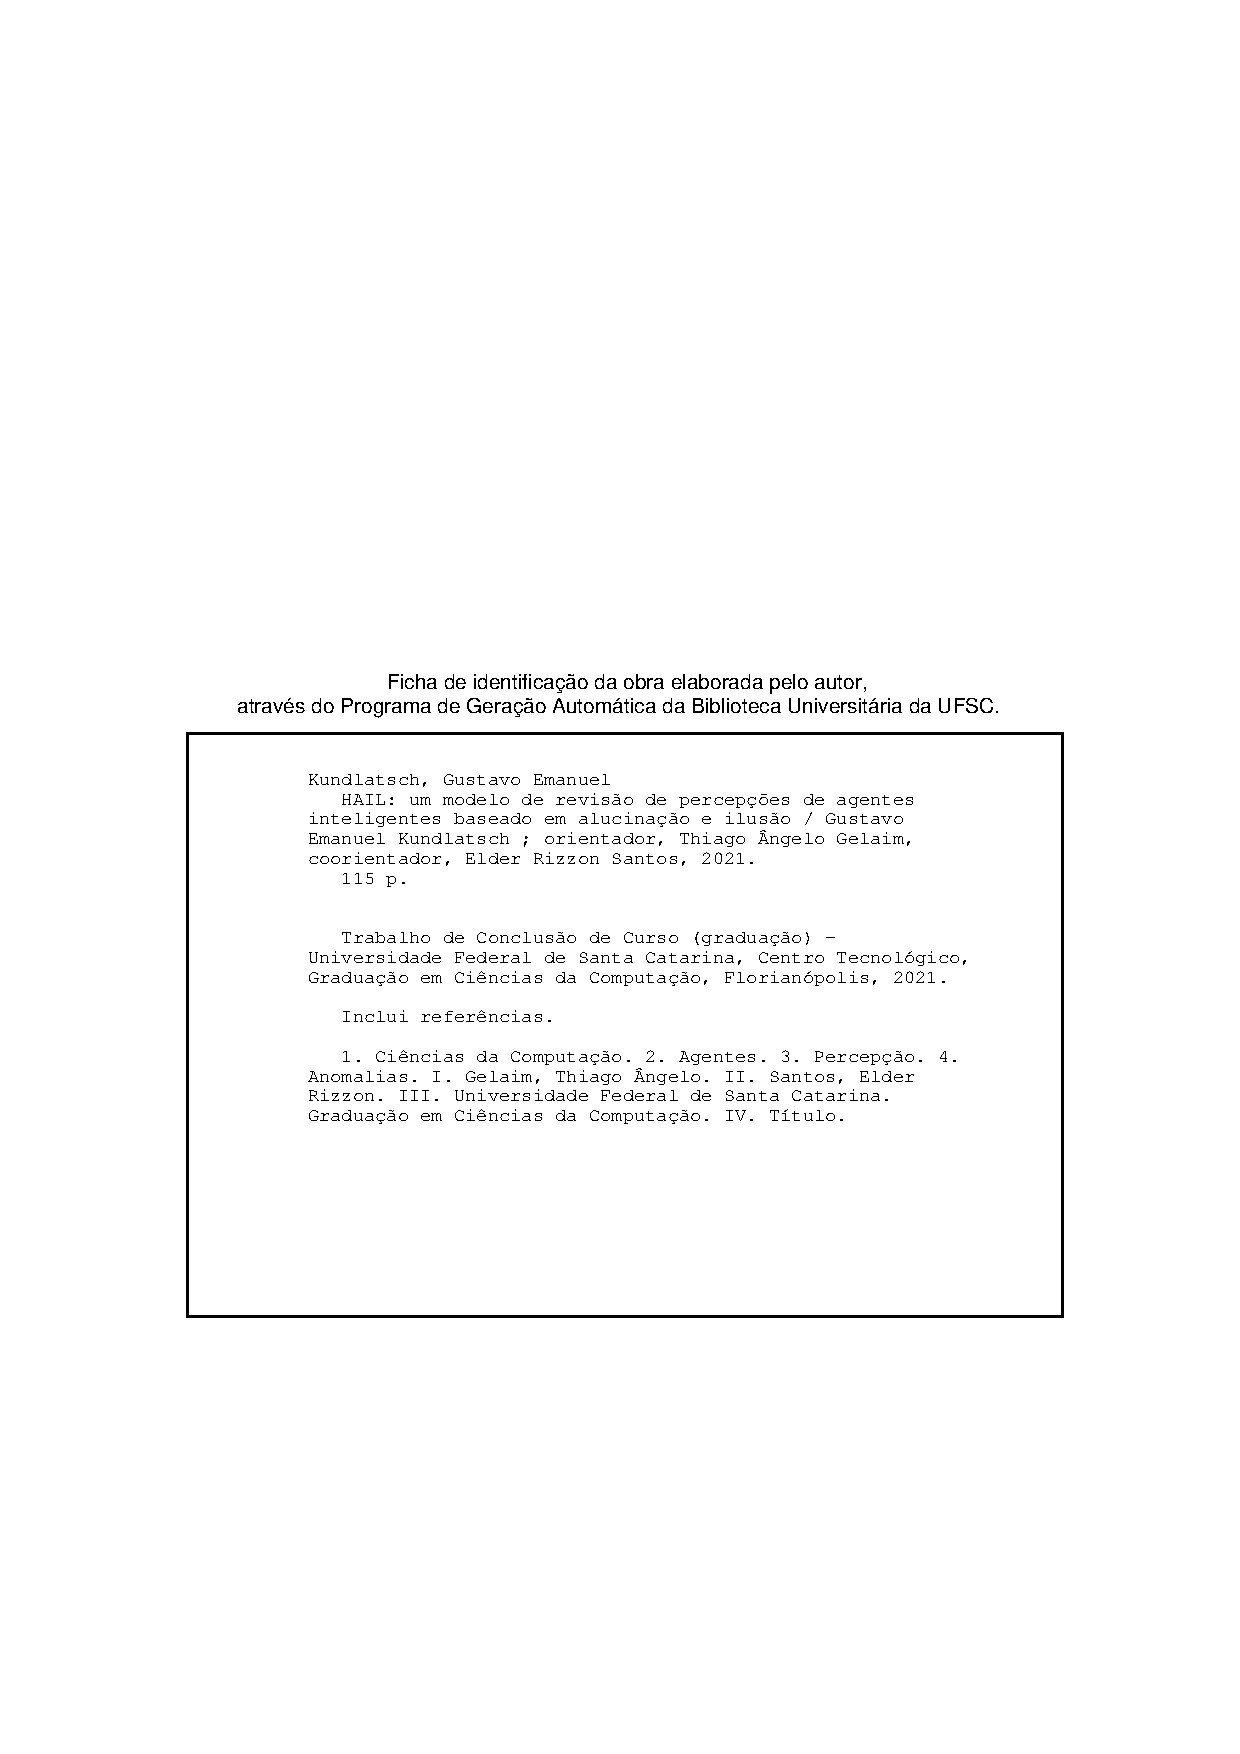
\includepdf{beforetext/Ficha_Catalografica.pdf}
% \end{fichacatalografica}
% ---

% ---
% Inserir folha de aprovação
% ---
% \begin{folhadeaprovacao}
% 	\OnehalfSpacing
% 	\centering
% 	\imprimirautor\\%
% 	\vspace*{10pt}		
% 	\textbf{\imprimirtitulo}%
% 	\ifnotempty{\imprimirsubtitulo}{:~\imprimirsubtitulo}\\%
% 	%		\vspace*{31.5pt}%3\baselineskip
% 	\vspace*{\baselineskip}
% 	%\begin{minipage}{\textwidth}
% 	O presente trabalho em nível de \imprimirnivel~foi avaliado e aprovado por banca examinadora composta pelos seguintes membros:\\
% 	%\end{minipage}%
% 	\vspace*{\baselineskip}
% 	Dr. Thiago Ângelo Gelaim\\
% 	Orientador\\
% 	\vspace*{\baselineskip}
% 	Prof. Dr. Elder Rizzon Santos \\
% 	Coorientador e Responsável\\
% 	\vspace*{\baselineskip}
% 	Prof. Dr. Rafael de Santiago\\
% 	\vspace*{\baselineskip}
% 	Me. Rodrigo Rodrigues Pires de Mello\\
% 	\vspace*{2\baselineskip}
% 	\begin{minipage}{\textwidth}
% 		Certificamos que esta é a \textbf{versão original e final} do trabalho de conclusão que foi julgado adequado para obtenção do título de \imprimirformacao.\\
% 	\end{minipage}
% 	%    \vspace{-0.7cm}
% 	\vspace*{\fill}
% 	\assinatura{\OnehalfSpacing Coordenação do Programa de Graduação}
% 	\vspace*{\fill}
% 	\assinatura{\OnehalfSpacing\imprimirorientador \\ \imprimirorientadorRotulo}
% 	%	\ifnotempty{\imprimircoorientador}{
% 	%	\assinatura{\imprimircoorientador \\ \imprimircoorientadorRotulo \\
% 	%		\imprimirinstituicao~--~\imprimirinstituicaosigla}
% 	%	}
% 	% \newpage
% 	\vspace*{\fill}
% 	\imprimirlocal, \imprimirano.
% \end{folhadeaprovacao}
% ---

% ---
% Dedicatória
% ---
\begin{dedicatoria}
	\vspace*{\fill}
	\noindent
	\begin{adjustwidth*}{}{5.5cm} 
		\raggedleft       
		À Maria, com amor. Minha companheira, amiga e por vezes revisora voluntária. Sua ajuda e motivação fez este trabalho comigo.
	\end{adjustwidth*}
\end{dedicatoria}
% ---

% ---
% Agradecimentos
% ---
\begin{agradecimentos}
    Agradeço a meus orientadores, sem os quais este trabalho não seria possível;
    Aos membros do SpaceLab, em especial a equipe do FloripaSat-2 pela ajuda e suporte;
    À minha família, especialmente minha mãe, que celebrou, reclamou, agradeceu e chorou comigo durante toda a graduação;
    À todos os servidores da UFSC, por manter e prover educação pública, gratuita e de qualidade;
\end{agradecimentos}
% ---

% ---
% Epígrafe
% ---
\begin{epigrafe}
	\vspace*{\fill}
	\begin{flushright}
		\textit{``O êxito precoce é um péssimo professor. Quando isso acontece, somos
                  recompensados por nossa falta de preparação e, quando nos vemos
                  no meio de uma situação para a qual devemos nos preparar, não somos capazes. Não sabemos como fazê-lo.'' \\
			(Chris Hadfield, An Astronaut's Guide to Life on Earth, 2013)}
	\end{flushright}
\end{epigrafe}
% ---

% ---
% RESUMOS
% ---

% resumo em português
\setlength{\absparsep}{18pt} % ajusta o espaçamento dos parágrafos do resumo
\begin{resumo}
	\SingleSpacing
	Satélites artificiais são projetos que demandam níveis elevados de confiabilidade de seus módulos. Apesar de alguns projetos permitirem atualizações posteriores a firmware e programas, são raros os casos onde é possível revisar e corrigir hardware. Por esse motivo a etapa de testes e AIV (\textit{Assembly, Integration, and Verification}) é crucial para a garantia de que o projeto não corra mais riscos do que os que são inerentes à área. Esses fatores são amplificados quando tratamos de \textit{CubeSats}, que possuem escopo e orçamentos menores quando comparados a grandes projetos governamentais e/ou comerciais. Este trabalho propõe a implementação de um sistema de \textit{workflows} hospedados na plataforma de controle de versionamento \textit{GitHub} que, aliados à funcionalidade GitHub Actions, permitirá a execução automatizada de testes no contexto dos planos de \emph{Assembly, Integration, and Verification}(AIV) da missão FloripaSat-2 e, posteriormente, análise e interpretação dos dados coletados de modo a obter resultados qualitativos e quantitativos da execução.
	
	
	\textbf{Palavras-chave}: CubeSat. Nanossatélite. FloripaSat-2. AIV.
\end{resumo}

% resumo em inglês
\begin{resumo}[Abstract]
	\SingleSpacing
	\begin{otherlanguage*}{english}
	    Artificial Satellites are projects that demand highly reliable modules. Despite some missions allowing post-deployment updates to firmware and software, cases where it is possible to perform hardware maintenance are rare. Because of this fact, the \textit{Assembly, Integration and Verification} (AIV) process is crucial to guarantee that the project doesn't face more risks than those which are inerent of a space mission. These factores are intensified when dealing with \textit{CubeSats}, that statistically have lower budgets and scope when compared to large scale governmental and/or commercial space missions. This article proposes the implementation of a test automation workflow system hosted at GitHub that will make use of the GitHub Actions tool to allow automated execution of tests during the AIV step of the FloripaSat-2 mission, and lastly, will allow collection and analysis of data in order to draw relevant conclusions regarding the execution.
	
	
		\textbf{Keywords}: CubeSat. Nanosatellite. FloripaSat-2. AIV.
	\end{otherlanguage*}
\end{resumo}
%% resumo em francês 
%\begin{resumo}[Résumé]
% \begin{otherlanguage*}{french}
%    Il s'agit d'un résumé en français.
% 
%   \textbf{Mots-clés}: latex. abntex. publication de textes.
% \end{otherlanguage*}
%\end{resumo}
%
%% resumo em espanhol
%\begin{resumo}[Resumen]
% \begin{otherlanguage*}{spanish}
%   Este es el resumen en español.
%  
%   \textbf{Palabras clave}: latex. abntex. publicación de textos.
% \end{otherlanguage*}
%\end{resumo}
%% ---

{%hidelinks
	\hypersetup{hidelinks}
	% ---
	% inserir lista de ilustrações
	% ---
	\pdfbookmark[0]{\listfigurename}{lof}
	\listoffigures*
	\cleardoublepage
	% ---
	
	% ---
	% inserir lista de quadros
	% ---
	\pdfbookmark[0]{\listofquadrosname}{loq}
	\listofquadros*
	\cleardoublepage
	% ---
	
	% ---
% 	inserir lista de tabelas
% 	% ---
	\pdfbookmark[0]{\listtablename}{lot}
	\listoftables*
	\cleardoublepage
	% ---
	
	
	% ---
	% inserir lista de abreviaturas e siglas (devem ser declarados no preambulo)
	% ---
	% ---------------------------------------------------
% ------ Lista de abreviaturas e siglas -------------
% ---------------------------------------------------

\begin{siglas}
  \item[ AIV ] \emph{Assembly, Integration, and Verification}
  \item[ CSA ] \textit{Canadian Space Agency}
  \item[ FlatSat ] Plataforma de testes para módulos CubeSat
  \item[ NASA ] \textit{National Aeronautics and Space Administration}
  \item[ SpaceLab ] Laboratório de Pesquisa em Tecnologias Espaciais - UFSC
  \item[ UFSC ] Universidade Federal de Santa Catarina
\end{siglas}
	% ---
	
	% ---
	% inserir lista de símbolos (devem ser declarados no preambulo)
	% ---
% 	% ---------------------------------------------------
% ----------- Lista de símbolos ---------------------
% ---------------------------------------------------

\begin{simbolos}
%   \item[$ \Delta $] Função de transição do modelo de revisão de percepções
%   \item[$ \Gamma $] Função de transição que especifica um sistema de transição de estados $\Sigma$
%   \item[$ \gamma $] Função de percepção do agente
%   \item[$ \theta $] Função de refinamento
%   \item[$ \rho $] Conjunto de percepções refinadas
%   \item[$ \Sigma $] Sistema de transição de estados de um modelo conceitual de planejamento automatizado
%   \item[$ \Psi $] Conjunto união formado pelas pré-condições das ações que compõem um plano
%   \item[$ \psi $] Conjunto de pré-condições de uma ação
%   \item[$ \Omega $] Conjunto união formado pelas pós-condições das ações que compõem um plano
%   \item[$ \omega $] Conjunto de pós-condições de uma ação
%   \item[$ A $] Conjunto finito ou recursivamente enumerável de ações
%   \item[$ Ab $] Conjunto de blocos avaliadores
%   \item[$ Ab_{h} $] Bloco avaliador de alucinações
%   \item[$ Ab_{i1} $] Bloco avaliador de ilusões classe 1
%   \item[$ Ab_{i2} $] Bloco avaliador de ilusões classe 2
%   \item[$ Ag$ ] Agente
%   \item[$ Ap $] Conjunto de blocos de planejamento automatizado
%   \item[$ Ap_{h} $] Bloco de planejamento automatizado de alucinações
%   \item[$ Ap_{i} $] Bloco de planejamento automatizado de ilusões
%   \item[$ c $] Contexto do agente
%   \item[$ Ce $] Função equação de limpeza do bloco avaliador
%   \item[$ Cf $] Função de limpeza do bloco avaliador
%   \item[$ D $] Conjunto de decisores
%   \item[$ d_{a} $] Decisor de anomalias
%   \item[$ d_{h} $] Decisor de alucinações
%   \item[$ d_{i} $] Decisor de ilusões
%   \item[$ E $] Conjunto finito ou recursivamente enumerável de eventos
%   \item[$ K $] Conjunto de conhecimentos do agente
%   \item[$ L $] Lista ordenada
%   \item[$ |L| $] Número de elementos de uma lista ordenada
%   \item[$ L_i $] Elemento $i$ da lista ordenada $L$
%   \item[$ M_{ai} $] Módulo de alucinação e ilusão
%   \item[$ P $] Conjunto de planos do agente
%   \item[$ p $] Conjunto de percepções iniciais
%   \item[$ P(L_i) $] Função peso da lista ponderada
%   \item[$ Pf $] Função de processamento do bloco avaliador
%   \item[$ S $] Conjunto finito ou recursivamente enumerável de estados
%   \item[$ T_{m}(x) $] Função tempo médio de x
%   \item[$ W $] Função peso de uma anomalia
%   \item[$ Z $] Descrição de sistema
\end{simbolos}


	% ---
	
	% ---
	% inserir o sumario
	% ---
	\pdfbookmark[0]{\contentsname}{toc}
	\tableofcontents*
	\cleardoublepage
	
}%hidelinks
% ---
% ---

% ----------------------------------------------------------
% ELEMENTOS TEXTUAIS
% ----------------------------------------------------------
\textual

\chapter{Introdução}
\label{chapter:introducao}
% \section{Introdução}
CubeSats são uma classe de artefatos espaciais elaborada com o intuito de reduzir custos e tempo de desenvolvimento, além de providenciar maior acessibilidade ao espaço \cite{cubesat-spec}. Inicialmente projetados para utilização educacional em universidades \cite{burt2011}, são amplamente usados para exploração espacial em órbita terrestre baixa, com altitudes entre 160km e 2000km \cite{alanazi2019}.

CubeSats possuem uma unidade básica (U) de dimensão 10cm x 10cm x 10cm e de até 1kg de massa, mas podem ser configurados em até 24 Unidades (ou 24U) \cite{cubesat}. O FloripaSat-2 \cite{floripasat2}, projeto do Laboratório de Pesquisa em Tecnologias Espaciais da UFSC no qual este trabalho se baseia, é um CubeSat 2U que se encontra no presente momento, em estágio de desenvolvimento ativo. A figura \ref{fig:floripasat2-diagram} apresenta uma renderização da configuração do FloripaSat-2.

\begin{figure}[H]
\caption{\label{fig:floripasat2-diagram}Renderização do FloripaSat-2.}
\begin{center}
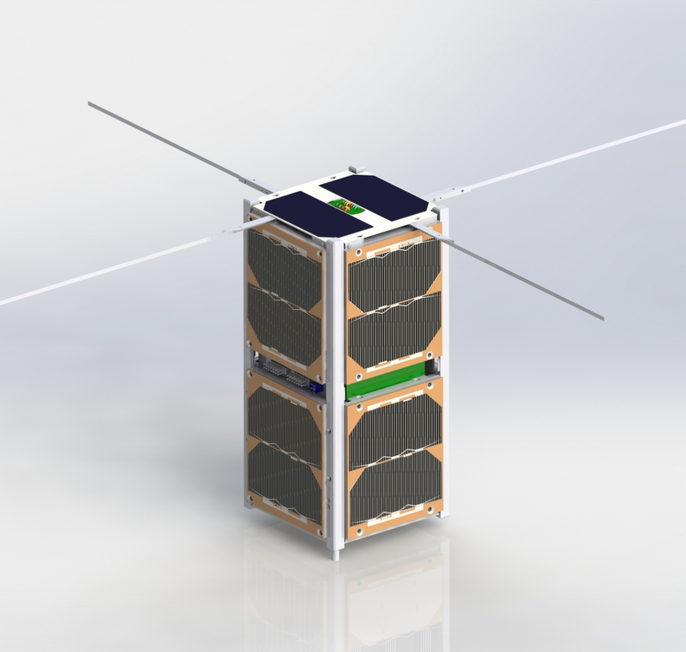
\includegraphics[scale=0.5]{images/floripasat-2-diagram.jpg}
\end{center}
\legend{Fonte: \cite{floripasat2}}
\end{figure}
\newpage

O processo de verificação de design é uma etapa crucial em projetos de engenharia.
Em tradução livre dos autores, Monteiro et al, dizem que:

\begin{citacao}
\hspace{1,2cm}Em projetos espaciais, a amplitude e cuidado minucioso dos processos de teste são ainda mais importantes, em vista do nível de confiabilidade  a ser imposto no produto final, que é comumente um artefato espacial que precisa resistir à uma gama de ameaças e funcionar em um ambientes inóspitos. \cite{aiv-cubesat}
\end{citacao}

Ainda segundo os autores, o processo de \emph{AIV} (sigla em inglês para Montagem, Integração, e Verificação) tende a ser mais leve em CubeSats, devido à menor escala dos projetos.

No entanto, o risco de um projeto de nanossatélite não é desprezível. Em um estudo realizado sobre os lançamentos de CubeSats entre 2003 e 2015, os autores \cite{panga2016} constataram que cerca de 15\% das missões CubeSat nesse período não conseguiram manter comunicações com as estações de controle, resultando em falha da missão após o lançamento.

Por esses motivos, percebe-se então a relevância de um plano de testes bem estruturado para o ciclo de desenvolvimento do FloripaSat-2. Através da elaboração e execução de testes, pretende-se elevar a confiabilidade\cite{chen-2001} do sistema, a fim de diminuir a probabilidade de que problemas no satélite resultem em falha da missão


O trabalho propõe, então, dois pontos principais:

\begin{itemize}
    \item A implementação de um sistema de workflows hospedados na plataforma GitHub Actions \cite {gh-actions} nos repositórios oficiais do projeto, que possibilite a execução automática de testes unitários nos sistemas do FloripaSat-2;
    \item A análise desritiva dos testes unitários implementados durante o desenvolvimento dos subsistemas do satélite.
\end{itemize}

Os resultados esperados deste trabalho são a criação de um modelo para automação a ser usado em futuros projetos de desenvolvimento de sistemas embarcados para CubeSats, e um relatório com as conclusões e análises obtidas por meio do estudo dos dados coletados.

\section{Objetivos}

\subsection{Objetivo Geral}

O objetivo principal do trabalho é implementar um sistema de automação dos testes unitários do firmware do FloripaSat-2 hospedado nos repositórios oficiais no \textit{GitHub}. Esses \textit{workflows} serão empregados durante o ciclo de desenvolvimento da missão, executando os testes de forma automática seguindo os critérios de execução estabelecidos pelo projeto.

\subsection{Objetivos Específicos}

\begin{enumerate}
    \item Apresentar uma introdução ao estado da arte referente a testes de software, desenvolvimento de CubeSats e relacionar os dois temas no contexto do FloripaSat-2;
    \item Implementar \textit{workflows} capazes de automatizar a execução de testes unitários;
    \item Apresentar um estudo sobre os testes dos sistemas do FloripaSat-2 que foram implementados durante o andamento do projeto;
    \item Disponibilizar códigos-fonte, dados de registro e resultados obtidos.
\end{enumerate}
\section{Organização do trabalho}

Este trabalho está organizado do seguinte modo:

\begin{itemize}
    \item O capítulo \ref{chapter:fundamentacao} apresenta a definição da metodologia utilizada e a formalização da fundamentação teórica utilizada na elaboração do trabalho;
    \item O capítulo \ref{chapter:relacionados} apresenta uma breve revisão de alguns trabalhos relacionados que abordam o desenvolvimento e testes de CubeSats;
    \item O capítulo \ref{chapter:proposta} apresenta e descreve o sistema proposto;
    \item O capítulo \ref{chapter:projeto} apresenta a descrição formal da implementação do sistema
    \item O capítulo \ref{chapter:resultados} apresenta uma análise dos resultados observados
    \item O capítulo \ref{chapter:conclusao} traz as conclusões e considerações sobre o trabalho, e explora possíveis trabalhos futuros
\end{itemize}

\chapter{Fundamentação teórica}

\label{conceitos-fundamentais}
Este capítulo apresenta a fundamentação teórica utilizada na elaboração do trabalho, trazendo conceitos básicos de nanossatélites
e automação de testes, além de um aprofundamento sobre como os temas foram empregados durante o desenvolvimento e implementação do trabalho.

\section{CubeSat}
\label{section:cubesat}
CubeSats são uma categoria de satélites miniaturizados cuja principal característica é possuir dimensões e massa reduzidos.
De acordo com o documento oficial de padrões de design\cite{cubesat-spec}, CubeSats devem ter estrutura em formato de cubo de
lado 100mm e não podem exceder 1kg de massa.

Essas características correspondem a uma unidade, ou um CubeSat 1U. Cubesats podem ser empilhados em múltiplas unidades, em
configurações como 2U, 3U, 6U ou 12U.

O padrão CubeSat foi desenvolvido pela \textit{California Polytechnic State University}, e é uma especificação de projeto de
colaboração internacional entre governos, universidades, escolas e o setor privado, com o principal objetivo de conceder acesso
ao espaço para cargas pequenas, e possibilitar missões com objetivos diversos, como demonstrações de tecnologia, como foi o caso
da missão Mars Cube One, desenvolvida pelo Jet Propulsion Laboratory e enviada à Marte \cite{mars-cubesat}, ou com objetivos
educacionais, como os CubeSats desenvolvidos pelo SpaceLab da UFSC.

Os CubeSats tradicionalmente possuem custo e risco baixos. Por serem fabricados em sua maioria com peças e materiais provienientes
de indústriais comvencionais, o orçamento de uma missão não se compara aos orçamentos bilionários de missões convencionais.
E do mesmo modo, o risco de se perder um CubeSat em uma missão que resulte em falha não é tão impactante em termos orçamentários e
de trabalho perdido. Esse fato faz com que esse tipo de missão seja ideal para ser utilizado com propósitos educativos por instituições
de ensino. A missão FloripaSat-1 da UFSC, por exemplo, teve como um dos objetivos treinar e capacitar estudantes de engenharia no processo
de desenvolvimento e operação de uma missão espacial \cite{marcelino2020-1}.

\section{Teste de Software}
Segundo Raul Wazlawick, quando se trata de teste é importante definir termos que, apesar de parecerem sinônimos, tem significados distintos
na área de testes de software:

\begin{itemize}
    \item error (error)
    \item defeito (fault)
    \item falha (failure)
    \item engano (mistake)
\end{itemize}

\section{CMocka}
CMocka is an elegant unit testing framework for C with support for mock objects. It only requires the standard C library,
works on a range of computing platforms (including embedded) and with different compilers.

\section{Mockups}
Mockups

\section{Automação de Testes}
\label{section:test-automation}

Durante o tempo de vida de um projeto de um software ou um sistema de softwares, como é o caso de um projeto de satélites artificiais,
os componentes envolvidos invariavelmente passarão por algumas mudanças. Mudanças essas que podem introduzir novos \textit{bugs} em
componentes que anteriormente funcionavam. A automação de testes, como definido pelos autores do livro
\textit{Software Test Automation - Effective use of test execution tools}, se dá pelo emprego de tecnologias que permitam que um caso
de teste seja executado de maneira autônoma, sem intervenção ou monitoramento, de maneira muito mais eficiente\cite{software-automation}
do que se executado via interação humana.

A etapa de testes é essencial em qualquer projeto de engenharia, e pode-se dizer que é ainda mais importante em projetos espaciais, já
que erros de projeto, sejam eles de hardware ou firmware, podem resultar em falha da missão.

Este trabalho propõe adotar a ferramenta de automação de testes em uma missão CubeSat, mais específicamente a FloripaSat-2, desenvolvida
pelo laboratório SpaceLab da Universidade Federal de Santa Catarina.

A FloripaSat-2 utilizará para testar e validar os seus subsistemas uma \textit{FlatSat}, descrita com mais detalhes na seção
\ref{section:flatsat}. O uso de \textit{FlatSats} tem um bom histórico de auxiliar na detecção e correção de erros e \textit{bugs},
como descrito por \cite{aiv-cubesat} e \cite{marcelino2020-2}. Por isso, julga-se que os bons resultados podem ser potencializados
por uma ferramenta de automação de testes, que permitirá a adoção de uma estratégia iterativa de desenvolvimento e correção de erros.

\chapter{Trabalhos relacionados}
\label{chapter:relacionados}

No motor de pesquisa acadêmica Google Scholar foram feitas pesquisas associando as áreas de conhecimento de desenvolvimento de nanossatélites, testes de software e automação de testes. As pesquisas foram realizadas ao longo da elaboração do trabalho e diferentes \textit{strings} de busca foram utilizadas. Como critério para escolha das publicações à serem estudadas, foram analisados os resultados apresentados na primeira página do motor de busca. Para determinar a relevância de uma publicação para o trabalho, foi analisado o \textit{abstract} e a introdução dos mesmos. Para os trabalhos relacionados apresentados neste capítulo os resultados e conclusõestambém foram estudados.


\begin{quadro}[h!]
\caption{Pesquisas realizadas}
\begin{tabular}{|l|l|}
\hline
\textit{String}          & Resultados \\ \hline
software+reliabilty+test & 565,000    \\
nanosattelite + design   & 15,200     \\
software + test          & 4,300,000  \\
software+test+automation & 1,970,000  \\
flatsat + cubesat        & 359        \\
cubesat                  & 29,200     \\
flatsat + nanosatellite  & 273        \\
cubesat + testbed        & 3,510      \\ \hline
\end{tabular}
 \label{quadro:pesquisas}
 \legend{Fonte: Autor.}
\end{quadro}

\section{Software Reliability Growth With Test Coverage \texorpdfstring{\cite{malaiya-2002}}{} }
\label{relacionados:malaiya-2002}
O termo "cobertura de testes", do inglês \textit{test coverage} quantifica o grau de rigor dos testes. Existem ferramentas que são capazes de mensurar a cobertura de testes em diferentes termos, como \textit{branches}, e inteção de uso. Os autores deste artigo trazem uma relação entre duração dos testes, cobertura e confiabilidade de software.

Desenvolvedores são capazes de atingir o nível de confiabilidade de \textit{software} de maneira previsível a partir de análise de confiabilidade durante o desenvolvimento. Para quantificar essa métrica durante os testes, o código é executado com \textit{inputs} selecionados aleatoriamente seguindo uma distribuição determinada. Dessa forma, se a distribuição utilizada for a mesma esperada durante a vida operacional do \textit{software}, pode ser levantado um modelo de confiabilidade a partir dos resultados dos testes.

Os autores constatam, no entanto, que para focar os testes na detecção de erros, é mais produtivo executar o código com \textit{inputs} considerados especialmente para estimular comportamentos onde erros são mais prováveis, e propõem neste estudo um modelo para realizar essa mensuração. Dentre os resultados obtidos na análise, os autores constatam que  em muitos casos, um mínimo de 85\% de cobertura de testes é necessário para aumento significativo na confiabilidade do software em desenvolvimento.

\section{How Do Software Developers Use GitHub Actions
to Automate Their Workflows? \texorpdfstring{\cite{kinsman-2021}}{} }
\label{relacionados:kinsman-2021}
Ferramentas sociais de programação, como o GitHub, alteraram a natureza colaborativa de desenvolvimento de \textit{software open source}, proporcionando novas oportunidades para engajamento, mas ao mesmo tempo aumentando a carga de trabalho de mantenedores de repositórios, que devem revisar, comunicar, explicar o projeto e gerenciar o versionamento de um número muito maior de colaboradores.

Para reduzir essa carga de trabalho intensiva, os autores estudam a ferramenta GitHub Actions, disponibilizada em 2019, que permite aos usuários automatizar questões como verificar se o código compila, se todos os testes são executados com sucesso, ou ainda se o código está dentro dos padrões de desenvolvimento do projeto. Esse controle pode ser feito segundo diversos \textit{triggers}, como \textit{commits}, comentários, \textit{issues} ou \textit{pull-requests}.

No artigo, os autores estudaram como desenvolvedores de software fazem uso da ferramenta para automatizar os fluxos de trabalho, como a ferramenta é discutida, e quais seus efeitos nos \textit{pull requests} dos projetos. Com uma amostra de 3,190 repositórios ativos no GitHub, e análise estatística de 926 deles, foi constatado que apenas uma pequena parcela dos repositórios utiliza a ferramenta, mas que a plataforma é vista, em geral, como benéfica para os contribuidores. Entre esses repositórios, os autores encontraram 708 \textit{workflows} de automação únicos.

Os autores relatam também que a utilização da ferramenta acarretou em diminuição da quantidade de aprovação de \textit{commits} mensal, e aumentou a quantidade de \textit{pull requests} rejeitados, experiências anedóticas revelam que a ferramenta e as funcionalidades que ela apresenta são recebidas com entusiasmo e apreciação pelos desenvolvedores.


\section{An Architecture-Tracking Approach to Evaluate
a Modular and Extensible Flight Software
for CubeSat Nanosatellites \texorpdfstring{\cite{gonzales-2019}}{}}
\label{relacionados:gonzales-2019}
Um ponto importante para aumentar o sucesso de missões CubeSat é a entrega de \textit{software} de vôo de qualidade. Esse tópico é identificado como chave para elevar a qualidade de diversos pontos de uma missão, como reusabilidade, colaboração, redução de riscos e facilitação de desenvolvimento. Uma arquitetura \textit{software} de vôo apropriada representa  os requisitos funcionais e não funcionais e guia o desenvolvimento. Dessa forma, para atingir o nível de qualidade desejada a arquitetura deve ser monitorada durante todo o ciclo de desenvolvimento de \textit{software}. Esse monitoramento, no entanto, é difícil e não-trivial.

Neste artigo, Gonzales \textit{et al.} apresentam detalhes sobre a implementação de missões CubeSat que se mostraram bastante similares à metodologia empregada no desenvolvimento do FloripaSat-2. Os autores trazem em seu trabalho pontos importanes sobre como entregar software de qualidade, confiável etolerante a falhas para missões CubeSat, que como toda missão espacial, se tratam de sistemas críticos que de modo geral devem operar de maneira autônoma e cujo software e hardware não podem ser corrigidos após o lançamento.

Os pontos de maior relevância para este trabalho são os requisitos não-funcionais de uma missão CubeSat trazidos pelos autores, entre eles a confiabilidade e extensibilidade do código, e a metodologia de projeto e arquitetura do \textit{software} de vôo, como a distinção entre as camadas do sistema, utilização de repositórios e em especial os métodos de validação utilizando métodos de integração contínua como ferramenta para elevar a confiabilidade do sistema através de testes automatizados.

Os temas apresentados pelos autores serão discutidos de forma mais profunda na \autoref{proposta:confiabilidade} e \autoref{projeto:floripasat2}.

\section{Integration and Verification Approach of ISTSat-1 CubeSat \texorpdfstring{\\ \cite{aiv-cubesat}}{} }
\label{relacionados:aiv-cubesat}
Satélites artificiais precisam resistir a uma grande quantidade de adversidades enquanto operam em um ambiente hostil e inóspito. Por isso é essencial que sejam feitos testes extensivos para garantir o nível de confiança necessário para que o objetivos da missão sejam atingidos. Porém, missões de CubeSat tendem a não ser tão rigorosas em suas etapas de montagem, integração e verificação (AIV), fato que é refletido na taxa de missões que acabam em falhas.

Esse paradigma, no entanto, está mudando a medida que a importância do CubeSats aumenta. Ela vai de simplesmente projetos educacionais, para missões de custos e importância elevados. Um exemplo desse salto é a missão Mars Cube One, ou MarCO \cite{mars-cubesat}, desenvolvida pelo \textit{Jet Propulsion Laboratory} da Nasa, que enviou dois CubeSats a Marte, para servirem como satélites de comunicação. Assim, os autores desse artigo apresentam a ideia de que integração e verificação em missões CUbeSats passam a ser encaradas com mais seriedade, como demonstrado na figura \ref{fig:nanosats_years_forecast}, onde é possível observar o aumento de lançamento de nanossatélites e, paralelamente, a diminuição da taxa de falhas.

Como estudo de caso, o artigo apresenta o processo de AIV empregado no desenvolvimento do ISTSat-1 \cite{istsat-1}, o primeiro nanossatélite português, lançado em 2021 e que utilizou a estratégia de teste através de uma \textit{FlatSat}, que se trata de uma plataforma de testes de \textit{Hardware In the Loop} (HIL).

A equipe do ISTSat-1, segundo os autores, optou por desenvolver a maioria dos subsistemas do satélite e adotou métodos ágeis para as atividades de AIV de forma a diminuir os riscos relacionados a falta de experiência da equipe. Dessa forma foi possível desenvolver e testar os módulos de forma contínua e iterativa, o que possibilitou a descoberta rápida de diversos erros e problemas que necessitavam de ajustes de design. Foi concluído nesse estudo que, caso a equipe tivesse optado por um processo de desenvolvimento em cascata, como tradicionalmente empregado em missões CubeSat, seria mais difícil, senão impossível, ter descoberto os mesmos problemas no design e funcionamento. Concluem então, que a adoção de processos iterativos é útil para projetos educacionais que contam com equipes sem muita experiência, ou sem muitos recursos financeiros.

\begin{figure}[h!]
    \centering
    \caption{Lançamentos anuais de Nanossatélites (previsão)}
    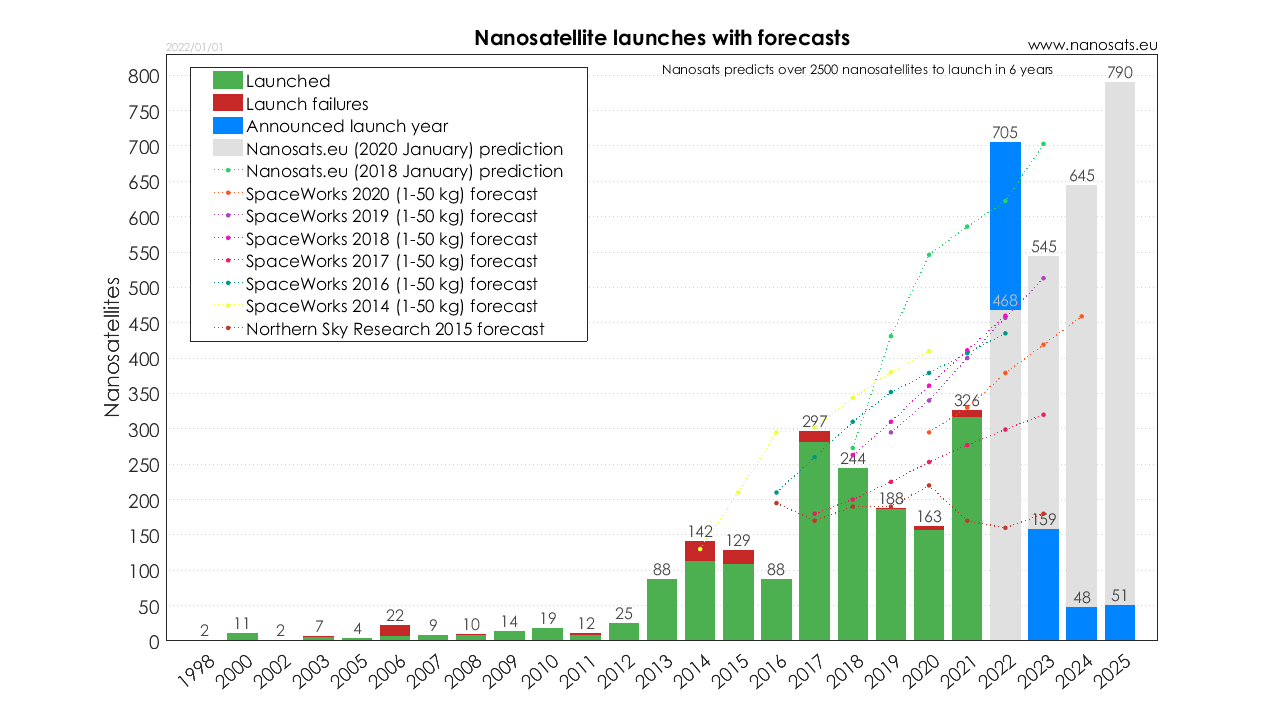
\includegraphics[width=\textwidth]{images/nanosat_years_forecast.png}
    \legend{Fonte: Nanosats Database \cite{nanosats-database}}
    \label{fig:nanosats_years_forecast}
\end{figure}


\section{Qualification and validation test methodology of the open-source CubeSat FloripaSat-I \texorpdfstring{\cite{marcelino2020-2}}{} }
\label{relacionados:marcelino2020-2}
Esta seção e a próxima apresentam dois trabalhos produzidos como resultado da missão FloripaSat-1, uma missão de demonstração desenvolvida inteiramente por estudantes da Universidade Federal de Santa Catarina (UFSC), cujo CubeSat foi lançado em 2019.

O FloripaSat-1 é composto de três módulos distintos, o sistema elétrico - EPS (\textit{Electric Power System}), o módulo de gerência de dados - OBDH (\textit{Onboard Data Handling}) e o módulo de telemetria e telecomandos - TT\&C (\textit{Telemetry, Tracking and Command}).

O artigo informa que a missão tinha como objetivo testar tecnologias que possibilitem o desenvolvimento rápido e de baixo custo de satélites espaciais, além de treinar estudantes nas áreas de concepção, implementação e operação de uma missão espacial completa. Além disso, o FloripaSat-1 é um projeto \textit{open source} e as informações de software e hardware dos módulos desenvolvidos estão disponíveis em repositórios públicos, para uso em futuras missões.

Os autores descrevem que o FloripaSat-1 foi desenvolvido com base em projetos de engenharia de sistemas, dividido em Modelos de protótipo (PM), engenharia (EM-I e EM-II) e finalmente o Modelo de Vôo (FM). Foram realizados testes em cada uma dessas etapas para validar os sistemas e os resultados, segundo o artigo, foram decisivos na detecção e correção de erros.

Apesar do artigo focar em integração e validação dos módulos a nível de hardware, julga-se relevante para a elaboração deste trabalho, que foca principalmente em software, por descrever as diferentes condições que uma missão espacial é submetida, além da metodologia de desenvolvimento adotada pela equipe do FloripaSat-1, em que a grande maioria dos membros seguiu para a missão FloripaSat-2, a qual este trabalho se baseia.

\section{A Critical Embedded System Challenge: The FloripaSat-1 Mission \texorpdfstring{\\\cite{marcelino2020-1}}{} }
\label{relacionados:marcelino2020-1}
Este artigo, elaborado também a partir da missão FloripaSat-1 do SpaceLab, apresenta definições e descrições dos subsistemas do satélite, além de algumas informações e resultados de testes e simulações realizadas nos mesmos.

Como descrito anteriormente, o FloripaSat-1 possui três sub sistemas principais:

\begin{itemize}
    \item \textit{Electric Power System} (EPS)
    \item \textit{On-Board Data Handling} (OBDH)
    \item \textit{Tracking, Telemetry and Command} (TT\&C)
\end{itemize}

O EPS é o módulo responsável por distribuir, coletar e armazenar a energia utilizada pelo satélite. A energia é coletada através de painéis solares e armazenada em uma bateria de íon de lítio. A distribuição da energia é definida a partir de um microcontrolador que analisa os estados de carga e de energia e decide quais módulos permanecerão em operação.

O OBDH é o módulo responsável pela gerência de atividades do satélite. Ele realiza a interface entre todos os subsistemas do satélite. Os dados gerados são empacotados e transmitidos através do TT\&C, e dados recebidos são enviados ao OBDH para que ele execute a tarefa requisitada, ou então envie o comando ao módulo requisitado. Este módulo também possui uma memória, para que possam ser futuramente recuperados.

Finalmente, o TT\&C é o módulo responsável pela comunicação entre o satélite e as estações de controle na Terra. Ele opera através de dois módulos de rádio, um para a banda VHF e um para UHF. Os comandos a serem enviados e recebidos pelo satélite (\textit{downlink}/ \textit{uplink}) são transmitidos através do módulo UHF e a banda VHF é reservada para transmissões do tipo \textit{beacon}.

Os autores discorrem ainda sobre os demais módulos e subsistemas do satélite, como outros \textit{payloads} que não foram desenvolvidos ou projetados pela equipe da UFSC e portanto, ficam de fora desse breve resumo.

A relevância deste artigo se dá pelo fato de que o FloripaSat-2 utiliza a mesma estrutura de subsistemas, com os seus módulos sendo sucessores diretos do software e hardware utilizados na missão anterior, operando de forma idêntica ou muito similar.


\section{In-orbit preliminary results from the open-source educational nanosatellite FloripaSat-I \texorpdfstring{\\\cite{marcelino2021}}{} }
\label{relacionados:marcelino2021}
O FloripaSat-I, como mencionado anteriormente, constituiu uma missão CubeSat desenvolvida na Universidade Federal de Santa Catarina, em que os objetivos incluiam testar tecnologias que permitissem desenvolvimento mais rápido e menos custoso de satélites futuros através do reuso da estrutura \textit{open source}. Lançado em 2019 em um foguete Chinês Long March 4B, os dados transmitidos pelo satélite foram usados como métricas de validação da missão, permitindo aos desenvolvedores (em sua maioria estudantes da UFSC) traçar paralelos entre os dados de órbita e as análises obtidas em laboratório.

Os autores apresentam uma análise dos resultados coletados durante os primeiros três meses da missão, além das lições aprendidas através dos dados recebidos.

O FloripaSat-I foi lançado em uma órbita heliossíncrona, que se trata de uma configuração de órbita quase polar, onde o plano de órbita é sempre fixo em relação ao Sol, e o objeto em órbita passa pela sobre a mesma região da superfície no mesmo instante todos os dias.\cite{tscherbakova-1998}.

Os dados enviados pelo satélite foram coletados em múltipas estações espalhadas pelo mundo, como apresentado na figura \autoref{fig:floripasat-stations}, e decodificados através de um \textit{software} de estação terrestre desenvolvido no laboratório.

\begin{figure}[h!]
    \centering
    \caption{Estações que receberam dados enviados pelo FloripaSat-I nos três primeiros meses da missão.}
    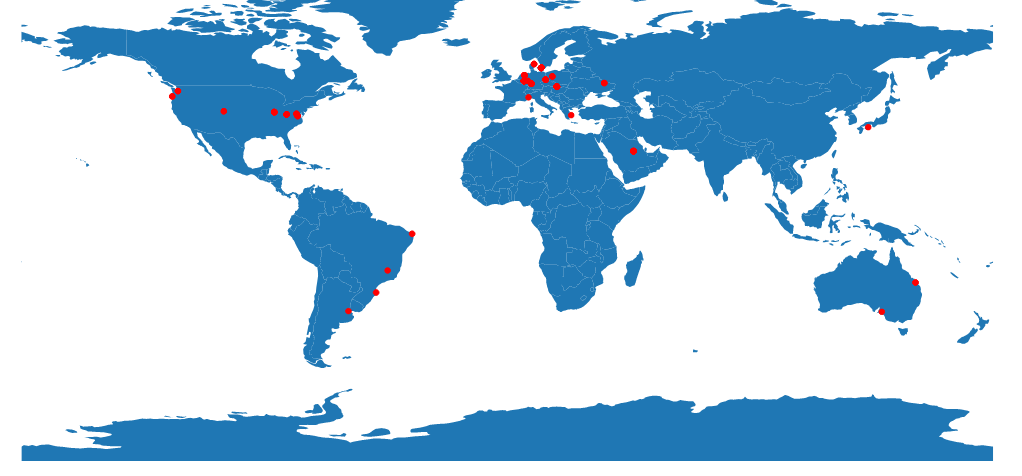
\includegraphics[width=\textwidth]{images/floripasat_stations.png}
    \legend{Fonte: \cite{marcelino2021}}
    \label{fig:floripasat-stations}
\end{figure}

No estudo publicado, os autores elencam algumas das dificuldades encontradas durante o desenvolvimento da missão e reveladas pelos dados do satélite em órbita, em especial dificuldades na montagem, que pode ter acarretado em problemas estruturais e de funcionamento, e de frequências utilizadas, que dificultaram a comunicação.

Além disso, foi realizada uma análise com os participantes do projeto com o intuito de compreender como a missão os afetou, e os resultados obtidos foram em geral percebidos como positivos pelos estudantes, que reportaram não apenas evolução de aprendizado e de experiência de desenvolvimento.

%

\section{Considerações}

Os artigos e teses escolhidos para embasar e fundamentar este trabalho estabelecem a importância de um modelo de testes bem estruturado em um projeto de desenvolvimento de \textit{software}. Todos os trabalhos relacionados a missões CubeSat mencionam a importância dos testes para a descoberta e solução de erros, bem como a relação entre a execução e planejamento dos testes e o aumento de confiabilidade do \textit{software.}, como demonstrado pelo estudo apresentado na \autoref{relacionados:malaiya-2002}.

O artigo apresentado na \autoref{relacionados:gonzales-2019} é especialmente interessante para a proposta desse trabalho por descrever em detalhes o processo e as práticas de desenvolvimento aplicadas na série de nanossatélites \textit{SUCHAI}, que se assemelham ao modelo proposto neste trabalho. Os autores citam diversos modelos e práticas de desenvolvimento que são, em essência, seguidos de maneira muito próxima pela missão FloripaSat-II, como será evidenciado no \autoref{chapter:proposta} e \autoref{chapter:projeto}.

O artigo analisado na \autoref{relacionados:marcelino2021}, apresenta uma análise dos resultados obtidos nos meses iniciais de operação do FloripaSat-I, bem como uma análise do impacto do satélite nos estudantes envolvidos no projeto. Este artigo demonstra as dificuldades encontradas no desenvolvimento da missão, e servem o propósito de indicar pontos de atenção e melhoria para trabalhos futuros, como é o caso do FloripaSat-II, que se inspira e por vezes diretamente reimplementa os sistemas utilizados no seu antecessor.

Além disso, os outros dois trabalhos produzidos por membros do SpaceLab, descritos na \autoref{relacionados:marcelino2020-1} e \autoref{relacionados:marcelino2020-2}, que relatam o processo de desenvolvimento da missão FloripaSat-1 mostram a importância de CubeSats como ferramenta educacional, servindo para treinar e capacitar estudantes no projeto, desenvolvimento e operação de uma missão espacial completa.

O modelo proposto por este trabalho é, então, uma continuidade dos pensamentos apresentados neste capítulo. Espera-se que o sistema implementado permita aumentar a qualidade e a confiabilidade do código entregue através de técnicas de integração contínua para automatizar os testes de unidade dos sistemas embarcados desenvolvidos para o FloripaSat-II, além de possibilitar mais uma ferramenta com potencial de estudo e aprendizado, sob a qual podem ser empregadas futuras ferramentas para analisar e expandir o modelo, como detalhado na \autoref{conclusao:futuros}.

\iffalse

\fi
\chapter{Fluxo de Automação de testes}
\label{chapter:proposta}
Este capítulo descreve e formaliza o sistema proposto. A motivação para este sistema surgiu a partir de reuinões e conversas com as equipes de desenvolvimento do FloripaSat-2 no SpaceLab, onde foi decidido adotar um modelo de testes que utilize nções de  integração contínua para automatizar o processo de publicar e testar os subsistemas desenvolvidos para o FloripaSat-2

O sistema proposto leva em consideração o ambiente de desenvolvimento, os objetivos da missão e as características do projeto para desenvolver um modelo cuja finalidade é facilitar e agilizar o ciclo de desenvolvimento, simultaneamente elevando a confiabilidade dos sistemas ao aumentar a cobertura de teste, como constatado por \cite{chen-2001}, cujo estudo apontou a correlação entre cobertura de teste e confiabilidade do software, como detalhado na \autoref{proposta:confiabilidade}


\section{visão geral do sistema}
\label{proposta:visao-geral}
O sistema proposto proporciona um ambiente de desenvolvimento onde os testes de software são executados de maneira automática e decentralizada, nos repositórios da missão FloripaSat-2. Essa abordagem proporciona, a princípio, dois pontos importantes:

\begin{itemize}
    \item A garantia de que toda alteração, adição ou remoção de código seja testada com a mesma precisão;
    \item Um ambiente transparente e universal para expor os testes executados e seus resultados.
\end{itemize}

A missão FloripaSat-2 possui três subsistemas próprios, desenvolvidos inteiramente no laboratório. Esses subsistemas estão descritos com mais detalhes na seção \ref{projeto:floripasat2}. Por esse motivo foi decidido durante o planejamento do sistema que seria necessário implementar um modelo que pudesse ser reproduzido de maneira simples e rápida em outros repositórios, para que todo código desenvolvido para a missão fosse tratado da mesma maneira. Para isso, foi implementado uma convenção de hierarquia de arquivos e nomenclatura, de modo a garantir a reusabilidade do modelo proposto, sem que seja preciso realizar grandes alterações. Como consequência, esse padrão acarreta em maior consistência entre os subsistemas do satélite. O padrão proposto está descrito em detalhes na \autoref{proposta:padrao}. No entanto, ele será melhor compreendido uma vez que se conheça o contexto de implementação. Por esse motivo, as próximas seções apresentam detalhes sobre funcionamento e implementação do modelo proposto.

\section{O Modelo}
\label{proposta:modelo}
A implementação dos subsistemas do FloripaSat-2 é hospedada nos repositórios da missão no GitHub. Por esse motivo foi decidido utilizar a ferramenta de CI/CD desenvolvida pela própria plataforma, a GitHub Actions\cite{gh-actions}, que proporciona um ambiente \textit{plug and play}, onde os \textit{workflows} são implementados e executados na própria plataforma, sem dependências externas.

O modelo foi pensado para possibilitar testar de maneira automática os sistemas embarcados do FloripaSat-2. Os módulos passam por testes unitários e análise estática, visando identificar e corrigir falhas e defeitos (melhor discutidos na \autoref{fundamentacao:testes}), e a partir disso elevar a confiabilidade do sistema de um modo geral, como exemplificado por \cite{chen-2001}.

Considerando esses pontos, os princípios básicos do modelo proposto são:

\begin{itemize}
    \item Testar os subsistemas de maneira automática
    \item Utilizar o GitHub Actions como hospedagem
    \item Ser facilmente transferido e implementado em outros projetos
\end{itemize}

\section{Funcionamento}
\label{proposta:funcionamento}

O modelo proposto se trata de um fluxo de execução constituído por três ações principais: a execução de um \textit{script} responsável por identificar e automatizar o processo; A compilação de arquivos fonte; e a execução dos arquivos compilados. Conforme elaborado na \autoref{projeto:analise}, o modelo se comporta de maneira diferente no caso de execução de Análise Estática. Nesses casos, o fluxo pode ser dividido em duas etapas: a execução do \textit{script} para identificar os arquivos fonte; e a análise estática destes mesmos arquivos.

O funcionamento detalhado do modelo é discutido em detalhes na \autoref{projeto:execucao}, mas de maneira breve, a execução de modo geral segue a seguinte cronologia:

\begin{enumerate}
    \item Um evento \textit{x} dispara a execução do script, que identifica os arquivos fonte \textit{y};
    \item Os arquivos \textit{y} são compilados, gerando binários executáveis \textit{z};
    \item Os binários \textit{z} são executados, e é gerado um relatório sobre o processo ao final da execução.
\end{enumerate}

Como um dos requisitos do modelo é a possibilidade de implementação em diferentes projetos, se faz necessário a padronização de alguns pontos dos projetos, de modo que as ações do fluxo de execução possam ocorrer com pouca ou nenhuma manutenção. O padrão desenvolvido está descrito na \autoref{proposta:padrao} a seguir.


\section{Padrão de Projeto}
\label{proposta:padrao}

De modo a garantir o funcionamento correto do modelo proposto em diferentes projetos, foi necessário padronizar o modo como o \textit{script} de automação identifica os arquivos relevantes. Para que isso aconteça, foi proposto um padrão de estrutura e nomenclatura de arquivos. Desta forma o sistema encontraria os arquivos sempre no mesmo local, e poderia a princípio ser simplesmente copiado para outros repositórios.

A título de compreensão do padrão, o trecho a seguir detalha a estruturação de um subsistema do FloripaSat-2, tomando como exemplo o commit \\ \textit{28c31e7a7db69240f1700ec3621436b14c517529} da branch \texttt{dev\_firmware} do repositório do OBDH 2.0\cite{obdh2-github}. A partir da raíz do diretório, o projeto é estruturado da seguinte forma\footnote{alguns arquivos e diretórios foram omitidos de modo a deixar o exemplo didático.}:

\begin{itemize}
    
    \item \textit{.github/workflows}
    
    \item doc
    
    \item firmware
    
    \begin{itemize}
        \item app
    
        \item config
    
        \item devices
        \begin{itemize}
            \item device 1
            \item device 2
            \item ...
            \item device n
        \end{itemize}
    
        \item drivers
        \begin{itemize}
            \item driver 1
            \item driver 2
            \item driver ...
            \item driver m
        \end{itemize}
    
    \end{itemize}
    \item hardware
    
    \item tests
    \begin{itemize}
        \item devices
        \item drivers
        \item mockups\footnotemark{}
    \end{itemize}
    
\end{itemize}
Ao padronizar a hierarquia de arquivos do projeto, obtem-se a garantia de que os \textit{scripts} sempre funcionarão corretamente, já que buscará os arquivos necessários sempre na mesma localização.
O outro aspecto do padrão estabelecido é a nomenclatura dos arquivos de teste, tanto arquivos fonte como os binários compilados. O padrão de nomenclatura foi definido da seguinte forma:



\begin{itemize}
    \item[] Arquivos de teste são nomeados \texttt{<alvo>\_test.c};
    \item[] Arquivos \textit{mockup} \footnotemark[\value{footnote}] são nomeados \texttt{<alvo>\_wrap.c}
    \item[] Executáveis são nomeados \texttt{<alvo>\_unit\_test}
\end{itemize}


\footnotetext{funcionamento e o propósito dos \textit{mockups} são descritos na \autoref{projeto:mock-object}}

\section{Confiabilidade}
\label{proposta:confiabilidade}
Foi demonstrado que testes e confiabilidade são muitas vezes temas correlacionados em engenharia e projeto de software\cite{malaiya-2002}.

Missões espaciais constituem sistemas críticos, e nanossatélites CubeSat não são exceção. Eles devem operar de maneira autônoma por anos, e em muitos casos sem oportunidade de manutenção à hardware e firmware. Entre os muitos requisitos não-funcionais que devem ser considerados em missões CubeSat, os autores Gonzales \textit{et al.} trazem esses fatos como razão para que os sitemas empregados em satélites sejam extensivamente testados de modo a mitigar a maior quantidade possível de possibilidades de falha. No entanto, devido à natureza de uma missão espacial, "atingir cobertura de código integral é impraticável na maioria dos casos"\cite{gonzales-2019}. Por isso, eles sugerem alguns outros modelos de desenvolvimento para reduzir pontos de falha, como por exemplo a implementação e utilização de um \textit{datapath} claro e simples, limitar o uso de \textit{mutexes} e alocação dinâmica de memória e, no caso do FloripaSat-2, optou-se por reduzir a utilização de numeração em ponto flutuante. A aplicação dessas \textit{guidelines} no FloripaSat-2 são analisadas na \autoref{projeto:floripasat2}

\section{Testes de Unidade}
\label{proposta:testes}
Os Testes de Unidade (do inglês \textit{unit tests}) são, como apresentado por Raul Wazlawick:
\begin{citacao}
\hspace{1,2cm}
"Os [testes] mais básicos e costumam consistir em verificar se um componente individual do \textit{software} (unidade) foi implementado corretamente. Esse componente pode ser um método ou procedimento, uma classe completa ou, ainda, um facote de funções ou classes de tamanho pequeno ou moderado. \cite{engenharia-software}.
\end{citacao}
Os testes de unidade são, segundo o autor, comumente implementados pelo próprio desenvolvedor, durante a produção do código. O objetivo desse modelo, e garantem pelo menos que "todos os comandos e decisões do componente implementado tenham sido exercitados para verificar se eles tem defeitos".

Os testes de unidade implementados para os subsistemas do FloripaSat-2 seguem os princípios e propósitos apresentados acima, e o modelo proposto visa fornecer uma plataforma para que os componentes desenvolvidos sejam testados de maneira automática e consistente, sempre que uma nova alteração é publicada.

Detalhes sobre a implementação dos testes de unidade para a missão FloripaSat-2 estão apresentados na \autoref{projeto:testes}, mas a princípio eles foram desenvolvidos para testar os \textit{devices}, implementações dos componentes presentes nos subsistemas do satélite, como por exemplos sensores de temperatura e corrente, e os \textit{drivers}, implementações de acesso ao \textit{hardware} dos subsistemas.

\section{Análise Estática}
\label{proposta:analise}

A análise estática, como colocada pelos autores Ayewah \textit{et. al.} (2008):

\begin{citacao}
\hspace{1,2cm}
Avaliam o \textit{software} no abstrato, sem executá-lo ou considerar um \textit{input} específico. Ao invés de tentar provar que o código cumpre suas especificações, estas ferramentas procuram por violações de práticas razoável ou recomendadas de desenvolvimento\cite{nathaniel-2008}
\end{citacao}

Ferramentas de análise estática são úteis também, segundo os autores, para "encontrar locais onde o código possa dereferenciar um ponteiro nulo, ou onde ocorra \textit{overflow} em \textit{arrays}"\cite{nathaniel-2008}.

A análise estática é empregada no desenvolvimento dos subsistemas do FloripaSat-2 através da ferramenta \cite{cppcheck}, que permite detectar problemas de \textit{undefined behaviour} e construções de código perigosas. A ferramenta também analisa código que não siga a sintaxe padrão da linguagem, como é comum em sistemas embarcados. Mais detalhes sobre o emprego e o funcionamento da ferramenta de análise sintática no FloripaSat-2 está descrita na \autoref{projeto:analise}.








\chapter{Implementação do Modelo}
\label{chapter:projeto}
    Este capítulo apresenta e detalha as implementações dos fluxos de execução hospedados no GitHub Actions e alguns dos testes unitários desenvolvidos, conforme mencionados no \autoref{chapter:proposta}.
    
    Para contextualização do modelo, bem como compreensão do ambiente de desenvolvimento, a \autoref{projeto:floripasat2} apresenta um detalhamento sobre a missão e como ela é dividia, em termos de desenvolvimento. Como discutido anteriormente, o FloripaSat-2 utiliza a filosofia Free Open Source Software, e portanto todos os módulos e subsistemas desenvolvidos estão publicados em repositórios abertos, no GitHub da missão. As seções \ref{projeto:eps}, \ref{projeto:ttc} e \ref{projeto:obdh} referenciam em seu texto os repositórios oficiais de cada um dos subsistemas desenvolvidos no SpaceLab.
     
    
    \section{FloripaSat-2}
    \label{projeto:floripasat2}
    
        Segundo Gonzales \textit{et. al.} (2019), "o \textit{software} de vôo de uma missão CubeSat constitui um dos elementos essenciais para garantia do sucesso da missão, já que é onde são implementados grande parte dos requisitos funcionais da missão". \cite{gonzales-2019}. Segundos os autores, é o que também permite que missões CubeSat sejam escaláveis e reutilizáveis.
        
        De fato, o FloripaSat-2 se beneficia destas propriedades. A missão é precedida pelo FloripaSat-1, lançado em dezembro de 2019, e como apresentado na \autoref{relacionados:marcelino2020-1}, segue a mesma metodologia e prática de desenvolvimento. Por consequencia, os módulos e substistemas, tanto \textit{hardware} como \textit{firmware} foram planejados para serem diretamente herdados do FloripaSat-1 ou atualizações de suas versões.
        
        Este trabalho foi em sua maioria focado nos subsistemas EPS 2.0 e OBDH 2.0 por estarem em estágios mais avançados de desenvolvimento, e os códigos-fonte discutidos e apresentados se encontram nos repositórios oficiais e públicos da missão, em \cite{eps2-github} e \cite{obdh2-github} respectivamente. Trechos relevantes do \textit{firmware} são apresentados e explicados neste capítulo, e apresentados em um contexto mais amplo nos anexos e apêndices ao final do documento. Por se tratarem de projetos relativamente grandes em questão de extensão de código, eles não foram anexados integralmente nesta monografia, que se beneficia do caráter público dos projetos do SpaceLab. Toda a implementação mencionada pode ser encontrada nos repositórios do FloripaSat-2 no GitHub\cite{floripasat2}.
        
        \subsection{EPS 2.0}
        \label{projeto:eps}
            O EPS 2 (\textit{electrical power system}) é responsável por coletar, armazenar e distribuir energia para o FloripaSat-2. A coleta de energia é feita através de 10 painéis solares posicionados ao longo da estrutura do satélite, e é armazenada em 4 baterias de íon de lítio. A distribuição de energia é feita através de conversores DC-AC. Tal qual o módulo desenvolvido para o FloripaSat-1\cite{marcelino2020-1} o EPS 2.0 possui um chip DS2775G+ utilizado para controlar carga e descarga da bateria, além de monitorar alguns parâmetros como corrente e tensão. O EPS, com base nessas informações, executa suas rotinas de distribuição de energia, decidindo quais módulos e quais funcionalidades devem permanecer em operação. O EPS 2 também é capaz de controlar a temperatura das baterias, e conta com sensores de temperatura e aquecedores.
            
            O projeto e implementação do EPS está disponível em seu repositório\cite{eps2-github}
            
        \subsection{TTC 2.0}
        \label{projeto:ttc}
            O módulo TTC 2 (Ou TT\&C, \textit{Telemetry, tracking \& Telecommand}) é o módulo de comunicação do FloripaSat-2. É função dele realizar a comunicação entre o satélite e a \textit{groundstation}. A comunicação com a estação terrestre será feita de duas maneiras, um sinal de \textit{beacon} e um de telemetria. 
            
            O \textit{beacon} transmite um sinal periódico contendo alguns dados básicos de identificação do satélite em conjunto com informações básicas de telemetria. O módulo de telemetria é o responsável pela comunicação de fato. Tém um módulo de comunicação bidimensional para receber telecomandos da Terra e transmitir os dados requisitados. O submódulo de telemetria é controlado por devices externos (como por exemplo o OBDH). 
            
            O projeto e a implementação do TTC 2 está disponível em seu repositório \cite{ttc2-github}.
        
        \subsection{OBDH 2.0}
        \label{projeto:obdh}
            O OBDH 2 (\textit{On-Board Data Handling}) é responsável pela sincronização as ações e o fluxo de dados entre os outros módulos do FloripaSat-2 e a groundstation. O OBDH organiza os dados em \textit{data frames} e transimte através do TTC, ou armazena em memória não-volátil para transimssão em outro momento. Dados recebidos da groundstation são captados pelo TTC e direcionados para o OBDH, que realiza a ação apropriada ou transmite para o módulo apropriado. 
            
            O OBDD também é responsável por sincronizar e fazer a interface entre os demais subsistemas do satélite, e para isso, de maneira similar ao módulo desenvolvido para o FloripaSat-1, o OBDH 2 utiliza como sistema operacional o \cite{freertos}. O sistema operacional de tempo real, nesse caso, é utilizado para garantir a execução das tarefas dentro dos limites de tempo estabelecidos, mesmo em caso de falhas \cite{marcelino2020-1}.
            
            O projeto e a implementação do OBDH 2 está disponível em seu repositório \cite{obdh2-github}.
    

    \section{Análise Estática}
    \label{projeto:analise}
        Como apresentado na \autoref{proposta:analise}, a análise estática de código fornece um meio de obter informações sobre o código desenvolvido, encontrar e corrigir erros potenciais sem precisar compilar o código, o que se mostra bastante benéfico em projetos complexos e interdependentes, como \textit{firmware} do FloripaSat-2. O uso de ferramentas de análise estática também garante maior precissão e segurança em códigos críticos.\cite{wichman-1995}. Segundo os autores, a análise estática tem duas características principais que devem ser mantidas em mente quando utilizadas: "natureza" e "profundidade" (\textit{nature} e \textit{depth}, no original):
        
        \begin{citacao}
        \hspace{1,2cm}
        natureza: é o objetivo amplo da análise, que pode ser adequação a algum padrão de linguagem, ou a corretude de algum aspecto em relação à especificaçao do programa;
        
        profundidade: indica a profundidade semântica da análise. Por exemplo, a análise de layout de um programa é rasa (...) enquanto provar um programa tem profundidade. \cite{wichman-1995}.
        \end{citacao}
        
        Wichman \textit{et. al.} relatam que análise estática é efetiva e complementar à testagem dinâmica, e seu uso é recomendado no desenvolvimento de sistemas críticos.
        
        Como mencionado na \autoref{proposta:analise}, os repositórios do FloripaSat-2 utilizam a ferramenta CPPCheck para análise estática de código, que verifica questões problemas com limites, tipagem, retornos e chamadas de funções. A lista completa de verificações feitas pode ser encontrada na página oficial da ferramenta, disponível em \cite{cppcheck}. Até o momento da escrita desta seção, a análise estática está implementada no módulo OBDH 2, onde é feita a verificação de todo o código implementado para o subsistema, com exceção dos testes. Seu uso foi configurado no modelo de automatização descrito na \autoref{proposta:modelo} e detalhado na \autoref{projeto:automacao}.
        
        

    \section{Testes de Unidade}
    \label{projeto:testes}
        \subsection{CMocka}
        \label{projeto:cmocka}
            Para a implementação dos testes de unidade nos módulos do FloripaSat-2, foi utilizada a ferramenta \cite{cmocka}, que implementa um framework de testes cuja única dependência é a biblioteca padrão C. Além disso, os testes escritos através da biblioteca são compilados em executáveis \textit{stand-alone} e, o mais importante para o projeto, suportam o uso de \textit{Mock Objects}, programas que simulam de maneira controlada o funcionamento de um sistema real. No caso do FloripaSat-2, os \textit{mockups} foram utilizados com o intuito de simular interações, dependências e chamadas \textit{I/O} de programas externos ao alvo do teste.
            
            Testes de unidade tem melhores precisão e eficiência quando empregados de maneira isolada e contida, para testar componentes e funcionalidades singulares. O componente sob teste deve ser analisado de maneira pura sem dependências e comunicações externas, pois isso acarretaria em introduzir código não testado para avaliar o funcionamento correto do componente desejado. Essa introdução pode trazer consigo \textit{bugs} e defeitos inesperados, para os quais o teste não está preparado para receber, impedindo o propósito do teste.
            
            De maneira simples, para testar um determinado componente \textit{a}, que depende dos componentes \textit{b} e \textit{c}, a melhor maneira de fazê-lo seria encontrar uma maneira de fazer com que \textit{a} possa contornar \textit{b} e \textit{c}, sem precisar que eles sejam invocados durante sua execução. Essa funcionalidade, a qual o prof. Raul Wazlawick nomeia \textit{stub} em seu livro \cite{engenharia-software}, é oferecida pela biblioteca Cmocka através dos \textit{Mock Objects} (\autoref{projeto:mock-object})
            
            \subsubsection{Um \textit{Mock Object} na CMocka}
            \label{projeto:mock-object}
                Como discutido anteriormente, a maior utilidade dos objetos \textit{mock} para o FloripaSat-2 é possibilitar a simulação de funções e componentes externos ao alvo do teste. Os \textit{Mock Objects} entram no projeto como forma de isolar o teste, de forma que qualquer erro ou defeito de implementação encontrado esteja localizado no próprio componente a ser testado.
                
                Dando continuidade ao exemplo iniciado na \autoref{projeto:cmocka}, ao escrever o teste para o componente \textit{a}, podemos criar um objeto \textit{mock} para os componentes \textit{b} e \textit{c}, de modo que sempre que \textit{a} realizar alguma chamada à \textit{b} ou \textit{c}, teremos controle sobre o envio e o retorno das chamadas, garantindo que somente o código de \textit{a} estará sendo executado, sem que bugs externos atrapalhem seu processo de teste.
                
                A CMocka utiliza a funcionalidade \texttt{--wrap} do ligador.
                o manual do \textit{GNU Linker} diz:
                
                \begin{citacao}
                --wrap=symbol
                
                \hspace{1,2cm}Utilize uma função \textit{wrapper} para \texttt{symbol}. Qualquer referência não definida à \texttt{symbol} será resolvida como \texttt{\_\_wrap\_symbol} (...)
                
                \cite{gnu-ld}
                \end{citacao}
                
                Segue então que, para testar de maneira isolada o componente \textit{a} devemos implementar funções \textit{mock} \textit{\_\_wrap\_b} e \textit{\_\_wrap\_c}. O teste de \textit{a} seria compilado, então, através do comando
                
                \begin{verbatim}
                    gcc a_test --wrap=b,--wrap=c
                \end{verbatim}
                
                Dessa forma, \textit{a} será compilado normalmente, mas chamadas à \textit{b} e \textit{c} serão resolvidas como chamadas aos seus respectivos \textit{wrappers}.
                
                Dentro de um arquivo de teste, essa interação é feita da seguinte maneira:
                
                Uma função que testa um componente que fará uma chamada à um \textit{wrapper} deve preparar anteriormente à execução do componente, o que a função \textit{wrapper} receberá e/ou retornará. No teste isso é feito através das funções \texttt{expect\_}. Consequentemente, a função \textit{wrapper} deve verificar a existência e a corretude do parâmetro enviado, através da função \texttt{check\_expected}. Essas duas funções permitem ao desenvolvedor e consequentemente ao próprio teste, saber de antemão qual o conteúdo das mensagens a ser trocadas, e qual o conteúdo das mesmas, podendo facilmente identificar se houve algum problema no percurso.
                
                Caso a função \textit{wrapper} deva retornar algum valor, isso pode ser feito dentro do teste através da função \textit{will\_return}, que especifica exatamente o que o \textit{wrapper} retornará, e o que vai ser recebido pelo componente testado. O \autoref{projeto:mock} dá continuidade ao exemplo anterior, exemplificando em código (relativamente) válido:
                
                \begin{lstlisting}[language=C, label=projeto:mock, caption=Exemplo de implementação e chamada de \textit{mock objects}]
                static void a_test (void **state) {
                    expect_value(__wrap_b, valor_b, 0);
                    will_return(__wrap_b, 1);
                    
                    expect_value(__wrap_c, valor_c, 1);
                    will_return(__wrap_c, 0);
                    
                    assert_return_code(a(0, 1), 0);
                }
                
                int __wrap_b(int valor_b) {
                    check_expected(valor_b)
                    return mock_type(int);
                }
                
                int __wrap_c(int valor_c) {
                    check_expected(valor_c);
                    return mock_type(int);
                }
                
                int a(int valor_b, int valor_c) {
                    int return_b = b(valor_b);
                    int return_c = b(valor_c);
                    
                    return 0;
                }
                \end{lstlisting}
                
                
                Exemplos dessas funções implementadas em testes reais no módulo EPS 2 do FloripaSat-2 estão apresentados nos trechos de código  \ref{projeto:__wrap_adc_read} e \ref{projeto:read_c_test}. 
                
                \lstinputlisting[language=C, label={projeto:__wrap_adc_read}, caption=\textit{Mock Function} do driver \textit{adc}, firstline=53, lastline=65]{code/adc_wrap.c}
                
                Neste trecho de código do arquivo \texttt{adc\_wrap.c} (disponível integralmente no apêndice \ref{apendice:adc}), É possível observar os mesmos princípios discutidos no exemplo anterior sendo aplicados na prática para testar os componentes. O \textit{ADC} nesse caso se refere à um conversor analógico-digital (\textit{analog-digital converter}).
                
                No EPS, o \textit{device} \texttt{temp\_sensor.c} utiliza o driver \textit{adc} para ler alguns sensores de temperatura, como parte da funcionalidade de controle térmico da bateria, conforme apresentado na \autoref{projeto:eps}. Dessa forma, para testar o temp\_sensor, foram implementadas funções \textit{wrapper} para todas as chamadas ao \textit{driver adc}.
                
                
                \lstinputlisting[language=C, label={projeto:read_c_test}, caption=função teste temp\_sensor, firstline=185, lastline=205]{code/temp_sensor_test.c}

    \section{Automação}
    \label{projeto:automacao}
        Como descrito anteriormente, o objetivo de automatizar a execução dos testes é potencializar os ganhos de confiabilidade nos sistemas desenvolvidos, além de garantir a corretude do código produzido através de uma cobertura de testes elevada. Esses objetivos foram almejados utilizando a ferramenta GitHub Actions, aproveitando-se do fato de que o desenvolvimento da missão já estava anteriormente hospedada no GitHub.
        
        \subsection{GitHub Actions}
            \label{projeto:gh-actions}
            Disponibilizada em 2019, GitHub Actions é uma API \textit{event-driven} para automatizar \textit{workflows} de desenvolvimento, que podem ser configurados para executar diversas atividades, a partir de diferentes tipos de eventos.
            
            Um evento, como definido pelos autores Kinsman \textit{et. al.}(2021): 
            \begin{citacao}
                \hspace{1,2cm} É uma atividade específica que dispara a execução de um \textit{workflow} (...) Por exemplo, um \textit{workflow} é disparado quando um \textit{pull-request} é criado, ou quando ocorre um \textit{merge} na \textit{branch} principal do repositório. \cite{kinsman-2021}
            \end{citacao}
            
            Os \textit{workflows} executados pela ferramenta são escritos em linguagem \textit{YAML}, e são implementados no diretório \texttt{.github/workflows}, na raíz do repositório.
            
            Um repositório pode ter um ou mais \textit{workflows}. De fato, os repositórios do FloripaSat-II, especialmente o módulog OBDH 2 \cite{obdh2-github}, contem três \textit{workflows} distintos: um para execução dos testes de unidade dos \textit{drivers}, o segundo com a mesma finalidade, para os testes de \textit{devices}, e um terceiro para a execução da análise estática do código. Após a execução dos \textit{workflows}, os resultados são apresentados em uma tela com \textit{logs}. Existem outras formas de tratar as mensagens de execução, mas a missão optou por visualizar as mensagens desta maneira, que não envolve outras configurações. A figura \autoref{fig:workflow-log} demonstra um exemplo de mensagem de \textit{log} após a execução com sucesso de um \textit{workflow} de testes.
            
            \begin{figure}[ht!]
                \centering
                \caption{Tela de resultados após a execução de um \textit{workflow}.}
                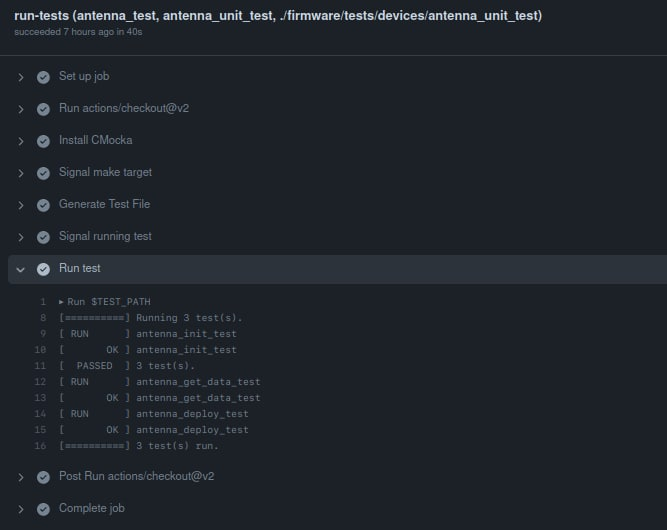
\includegraphics[width=\textwidth]{images/workflow_log.jpg}
                \label{fig:workflow-log}
                \legend{Fonte: OBDH 2 \cite{obdh2-github}}
            \end{figure}
            
            Os \textit{workflows} nos repositórios da missão são organizados em duas etapas distintas, separadas em Pré Execução \autoref{projeto:pre-exec} e Execução propriamente dita \autoref{projeto:exec}.
        
        \subsection{Pré Execução}
        \label{projeto:pre-exec}
            Na etapa de Pré Execução, são realizadas algumas tarefas para preparar o \textit{workflow}. Configurações iniciais, como escolha de sistema operacional e download e instalação de pacotes necessários foram omitidas, por se tratarem de configuração padrão da ferramenta, e não tem relevância para a execução do modelo desenvolvido.
            
            A primeira tarefa é a elaboração de uma \textit{Job Matrix}, que se trata de uma estrutura de dados empregada pela ferramenta para estabelecer um conjunto de \textit{jobs}, como são chamadas as ações da ferramenta. Um exemplo \textit{job}, no contexto do FloripaSat-II, seria um teste a ser executado. A \textit{Job Matrix} é utilizada, então, para dividir o \textit{workflow} de modo que cada arquivo de teste seja encapsulado em uma sub-tarefa distinta, que são executadas de maneira paralela. Optou-se por esse modelo como maneira de garantir execução e análise eficientes de e de maneira independente. A \autoref{tab:driver-tests} e a \autoref{tab:device-tests} apresentam uma comparação entre as execuções do workflow no repositório do OBDH 2.0 atual, e uma versão sequencial implementada especialmente para este teste.
            
            %%%%%%%%%%%%%%%TABELA%%%%%%%%%%%%%%%%%
\begin{table}[ht!]
\centering
\begin{tabular}{|l|l|l|l|}
\hline
\textbf{Modo de Execução  }    & \textbf{Min} & \textbf{Max}  & \textbf{Média} \\ \hline
Sequencial            & 38  & 69   & 50.27  \\ \hline
Paralela (Job Matrix) & 74  & 434\footnotemark & 128  \\ \hline
\end{tabular}
\caption{Tabela comparativa de tempos de exeução em segundos do workflow de testes unitários dos \textit{drivers} do OBDH 2.0}
\label{tab:driver-tests}
\end{table}
            %%%%%%%%%%%%%%%TABELA%%%%%%%%%%%%%%%%%
            
\begin{table}[ht!]
\centering
\begin{tabular}{|l|l|l|l|}
\hline
\textbf{Modo de Execução }     & \textbf{Min} & \textbf{Max} & \textbf{Média} \\ \hline
Sequencial            & 27  & 79  & 47.2  \\ \hline
Paralela (\textit{Job Matrix}) & 57  & 105 & 72.8  \\ \hline
\end{tabular}
\caption{Tabela comparativa de tempos de exeução em segundos do workflow de testes unitários dos \textit{devices} do OBDH 2.0}
\label{tab:device-tests}
\end{table}
        %%%%%%%%%%%%%%%TABELA%%%%%%%%%%%%%%%%%
        
            \footnotetext{O tempo de duração de 434 segundos foi possivelmente uma anomalia decorrente de alguma instabilidade na plataforma, visto que nenhuma das outras 10 execuções desse mesmo módulo apresentou valores próximos a este. Para fins de comparação, foi realizada uma nova medição desse mesmo workflow, e a média recalculada descartando o valor anômalo foi de 97.4 segundos. A lista completa das execuções pode ser encontrada nas tabelas \ref{tab:driver-tests-full} e \ref{tab:device-tests-full} no apendice \ref{apendice:tabelas}}
            
            O \textit{workflow} que implementa a execução sequencial dos testes se mostrou comparativamente mais rápido à execução paralela. A razão da escolha do uso da \textit{Job Matrix} foi a possibilidade de granularizar a execução, controlando de maneira individual se um teste deve ou não ser executado, além de ser possível analizar os resultados da execução de maneira individual. Como cada item da matriz é visualizada como um \textit{workflow} separado nos logs do GitHub, se torna trivial encontrar o teste desejado e analizar o resultado de sua execução. Na forma sequencial, por exemplo, a execução se dá em um único \textit{workflow}, e os testes e resultados devem ser buscados no log.
            
            Nesse contexto, um \textit{job} principal faz o levantamento de todos os arquivos de teste disponíveis para serem executados, e para cada arquivo é gerada uma entrada na \textit{job matrix}, de modo que cada teste seja compilado e executado em um \textit{job} isolado.
            
            O trecho de código \autoref{projeto:unit-test-devices} representa a seção do \textit{workflow} responsável por gerar o conteúdo da \textit{Job Matrix}, que no caso é populada com informações sobre os testes a serem executados.
            
            \lstinputlisting[language=yml, label={projeto:unit-test-devices}, caption=Geração da Job Matrix no workflow de autmação dos testes de \textit{devices} do OBDH, firstline=38, lastline=64]{code/unit-test-devices.yml}
            
            
            A execução desta etapa, que por sua vez invoca um script Python que lê o diretório onde o teste está implementado, cuja localização no repositório é informada no momento da execução. Assim, cada \textit{workflow} informa o caminho desejado. Por exemplo, no caso do OBDH 2.0, o workflow de \textit{drivers} informaria o caminho \texttt{firmware/tests/drivers}, enquanto o workflow de \textit{devices} deverá informar \texttt{firmware/tests/devices}. Essa configuração deve ser feita de forma manual na implementação dos \textit{workflows} individuais, e segue o padrão estabelecido e descrito na \autoref{proposta:padrao}.
            
            A execução deste script resultará em uma lista no formato \textit{.json} com os seguintes componentes:
            
            \begin{itemize}
                \item \textit{name}: o nome do arquivo de teste fonte.c, \textit{sem a extensão};
                \item \textit{test\_name}: o nome do executável após a compilação do arquivo fonte;
                \item \textit{path}: o diretório onde se encontra o executável;
            \end{itemize}
            
            Um exemplo desta lista gerada pelo workflow de \textit{devices} do OBDH 2.0 está disponível no trecho de código \autoref{projeto:test-list}.
            
            \lstinputlisting[language=json, label={projeto:test-list}, caption=Lista de testes gerada pelo script de identificação de arquivos, firstline=2, lastline=17]{code/test-list.json}
        
            O arquivo \textit{.json} apresenta o resultado da execução do script, onde cada elemento de \textit{include} é um dicionário contendo o nome do arquivo fonte, o nome e a localização do executavel.
            
            Esse arquivo é lido nos próximos passos do workflow para gerar os \textit{jobs} individuais com cada um desses dicionarios, dessa forma cada \textit{job} lida apenas com um executavel.
            
        \subsection{Execução}
        \label{projeto:exec}
            Após as configurações realizadas na etapa de Pré Execução, o \textit{workflow} realiza a compilação e a execução dos arquivos listados anteriormente, localizados no arquivo \textit{.json} gerado.
            
            Para efeitos de ilustração, assumiremos um commit na branch \textit{dev\_firmware} do repositório do OBDH 2 como evento \textit{e}, que aciona a execução de um \textit{worklow} \textit{w}.
            
            Após a etapa de Pré Execução, todos os arquivos de teste dos \textit{drivers} e \textit{devices} do OBDH2 estarão listados no arquivo \textit{.json}, e a \textit{Job Matrix} estará populada com os nomes e os caminhos de cada um deles. Cada entrada na matriz é, então, dividida em uma sub tarefa.
            
            Como cada tarefa é encarada como um \textit{workflow} distinto sob o ponto de vista de execução, todas elas precisam realizar algumas configurações iniciais como as descritas anteriormente, de download e instalação de bibliotecas. Após isso, o teste é compilado, e o binário gerado é executado. Ao final da execução, um registro com informações sobre o \textit{workflow} é gerado (\autoref{fig:workflow-log}).
            
            Caso algum dos testes apresente falha, o \textit{workflow} registrará um erro de execução, mas isso ocorrerá apenas após a finalização de todos os testes.
            
            A \autoref{fig:workflow_chart} ilustra um fluxo de execuções seguindo as etapas discutidas nas últimas seções.
            
            
\begin{figure}[h!]
    \centering
    \caption{Fluxo de execução do modelo de automação}
    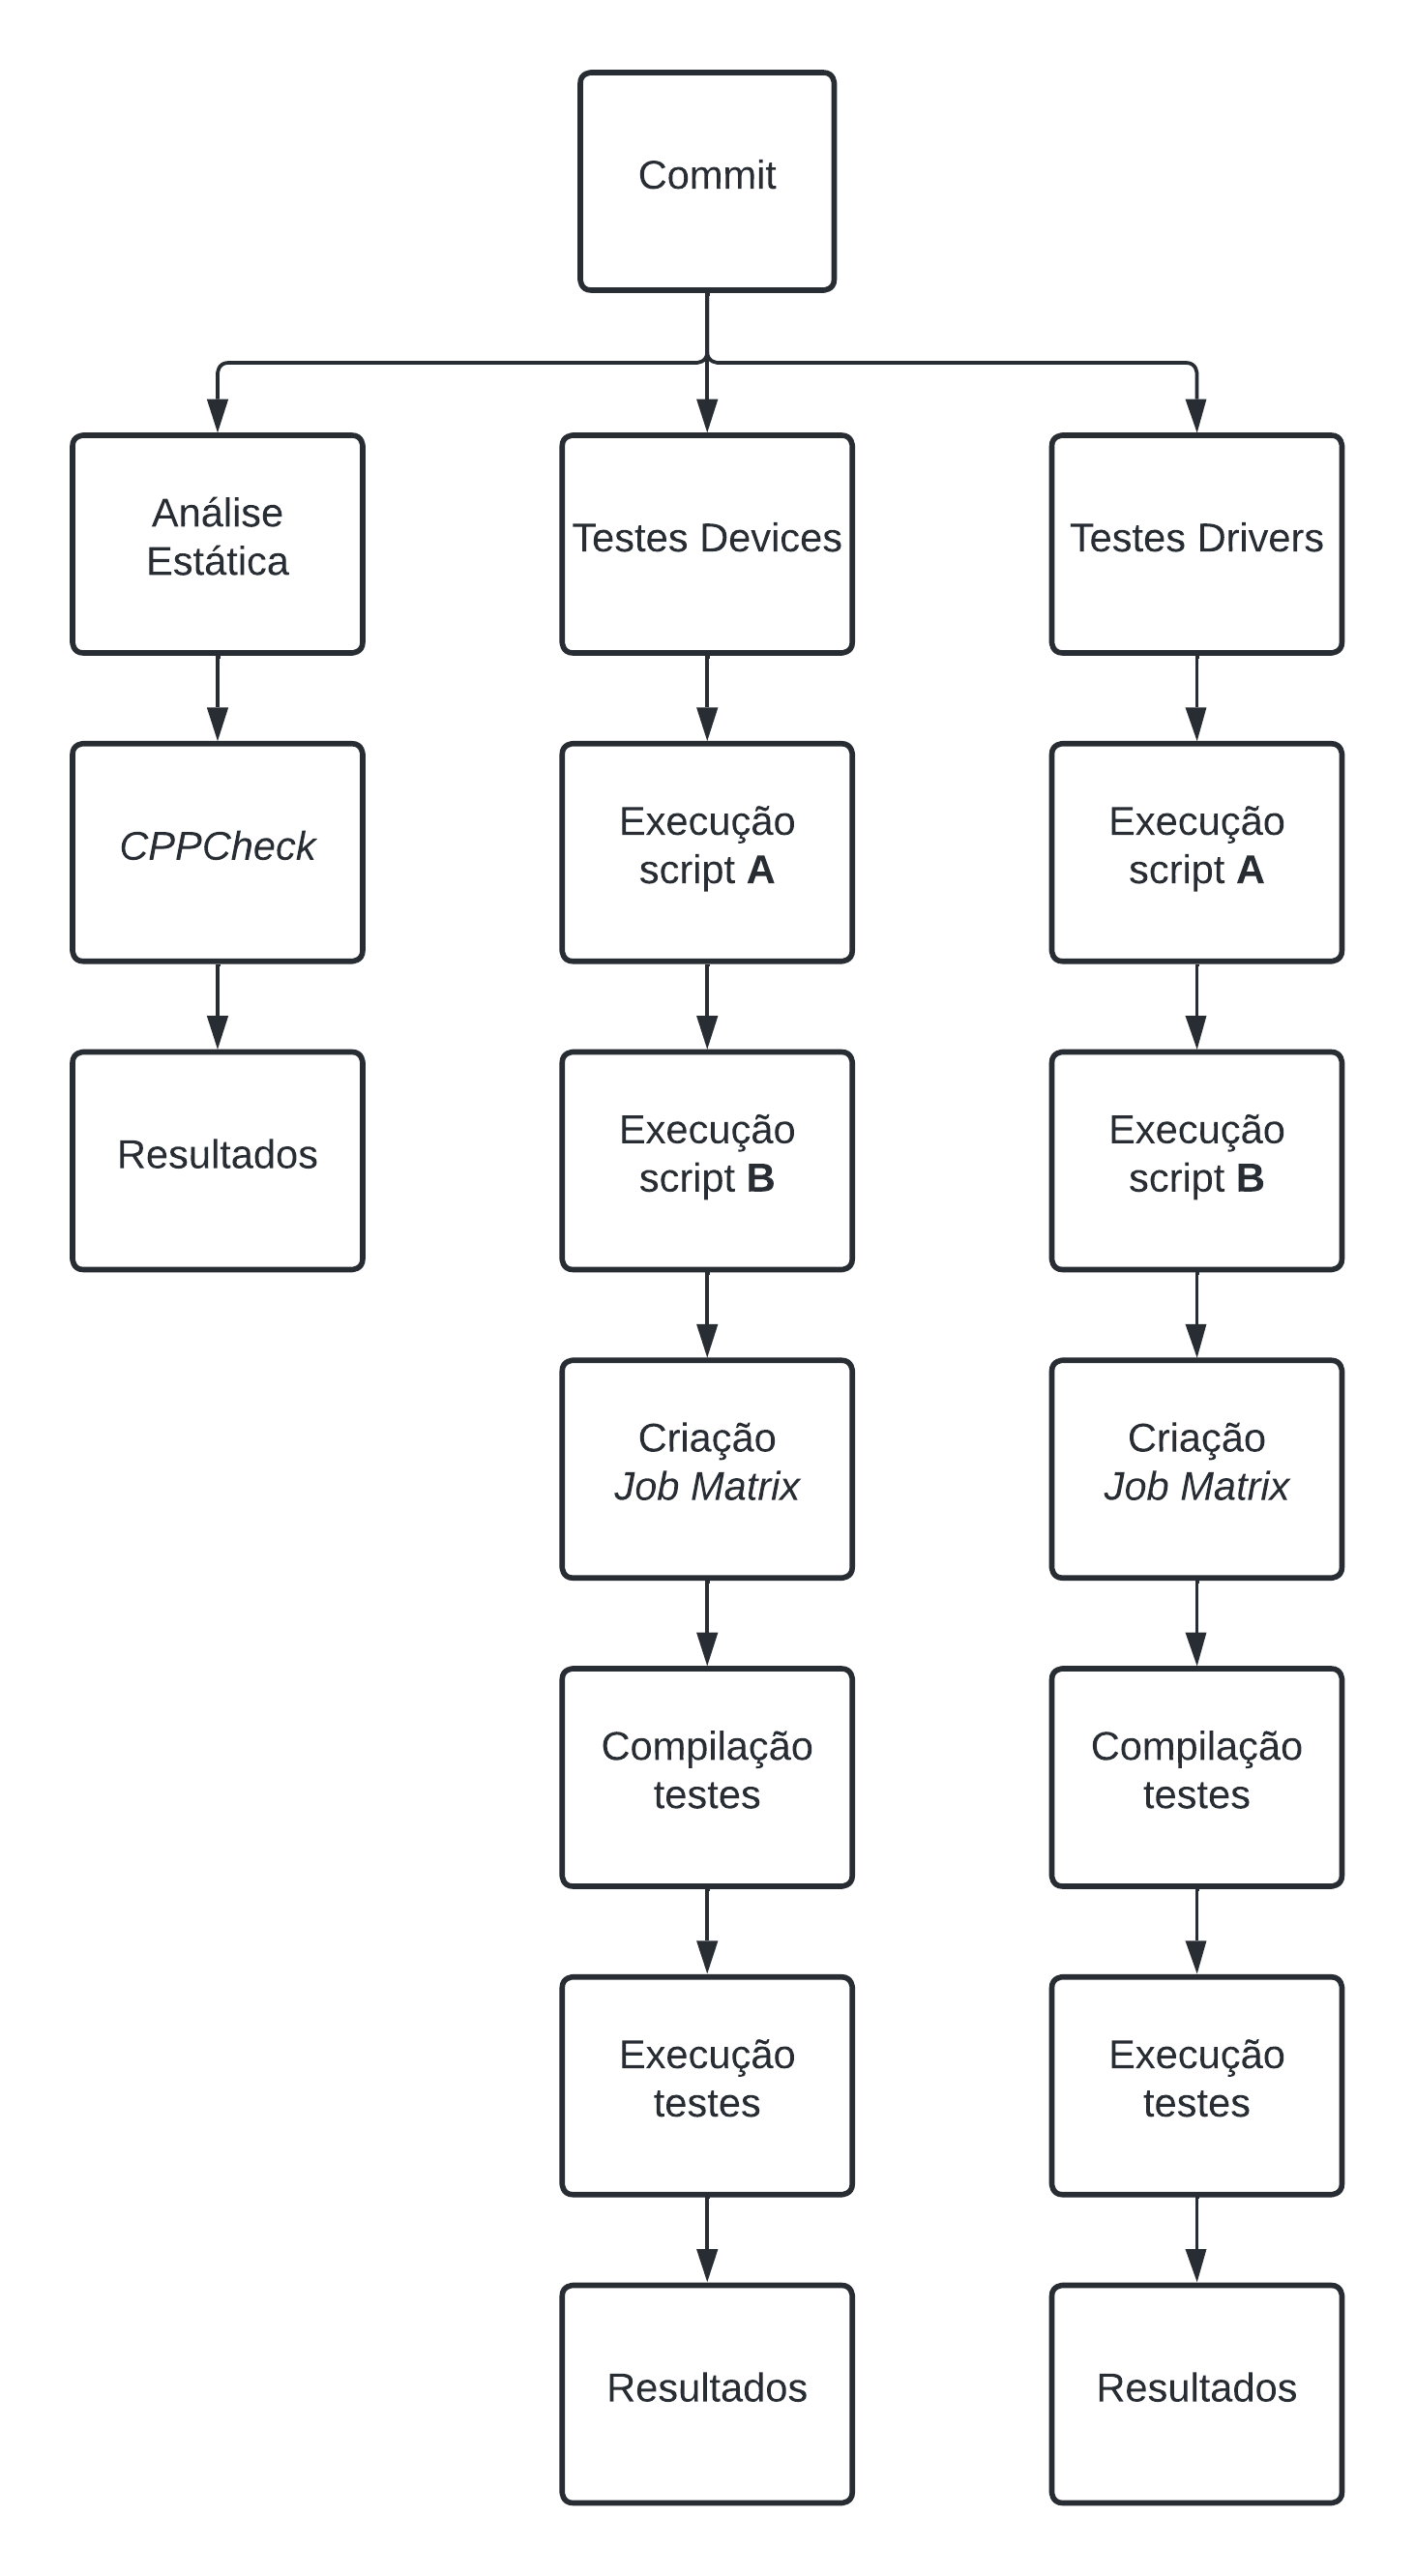
\includegraphics[scale=.15]{images/workflow_chart.png}
    \legend{Fonte: O autor}
    \label{fig:workflow_chart}
\end{figure}
\chapter{Resultados}
\label{chapter:resultados}

    \section{Execuções}
    \label{resultados:execucoes}
    Os workflows no repositorio do obdh (onde os testes já estão mais consolidados) foram executadas 447 vezes até a data da escrita deste trabalho, sendo que 44 execuções representaram falhas. O que representa cerca de 10\% das execuções.
    
    No EPS, 77 execuções com 15 falhas, uma taxa de aproximadamente 20\%. O Número de execuções é menor, e a taxa de falhas é maior, porém o eps2 está em desenvolvimento ativo, com os testes ainda sendo escritos e implementados.
    
    \section{Bugs encontrados}
    \label{resultados:bugs}
    
    \section{Considerações}
    \label{resultados:consideracoes}
    Os workflows foram amplamente utilizados durante os ciclos de desenvolvimento do FloripaSat-2 e serviram ativamente para encontrar e solucionar problemas na implementação.
\chapter{Considerações finais}
\label{chapter:conclusao}

    Os trabalhos relacionados escolhidos \autoref{chapter:relacionados} apresentam um panorama inicial bastante informativo, quando analizados em conjunto:
    \begin{itemize}
        \item A relevância de missões CubeSat cresce a cada ano, observada pelo crescente volume de lançamentos;
        \item São projetos com potencial educacional elevado, sendo usados por insituições de ensino para capacitar e treinar estudantes e também desenvolver, testar novas tecnologias e processos de desenvolvimento.
        \item Se tratam de sistemas críticos, cuja confiabilidade é fator essencial para o sucesso da missão
    \end{itemize}
 
    Os artigos elaborados pela equipe do FloripaSat-I demonstram a enorme quantidade de conhecimento gerada, bem como a experiência adquirida em projeto e desenvolvimento de tecnologias espaciais. Os resultados preliminares obtidos após o lançamento do FloripaSat-I também se mostraram essenciais, ao revelar pontos de atenção e dificuldades a serem melhor tratados na missão atual.

    Percebeu-se também que, embora exista uma biblioteca ampla sobre testes de hardware de \textit{CubeSats}, a quantidade de material distinto que foque apenas (ou principalmente) em teste de software espacial é comparativamente menor. O material encontrado, no entanto, revela os benefícios e melhorias que o modelo proposto por esse trabalho potencialmente proporciona. Espera-se que esse trabalho seja entendido como uma continuidade desse pensamento, no estudo realizado nos testes de unidade do FloripaSat-II.

    O estudo destes trabalhos relacionados evidência também a importância de um projeto de testes estruturado. Mais de uma vez, nos artigos selecionados anteriormente foi descrito que a etapa de testes foi importante para a descoberta e correção de erros de design, sejam eles de harware ou software. É nessa vertente que este trabalho propôs e implementou uma nova aproximação para os testes unitários do FloripaSat-2, por meio de um sistema de workflows que permite a execução de testes de maneira automática.
    
    É possível verificar a importância da execução destes \textit{workflows}, que permitem a centralização e a transparência dos testes escritos, de uma forma que seja facilmente identificável quando um erro de implementação ocorra, e igualmente fácil a todos os desenvolvedores analisarem e terem a oportunidade de contribuir com a identificação e correção dos erros.
    
    Além disso, publicações e entregas de código podem ser agilizadas, sendo que uma vez que os testes já estejam escritos e implementados no repositório, os commits podem ser feitos de forma experimental, e o \textit{workflow} apresentaria um relatório, apontando se e quais falhas foram implementadas.
    
    \section{Trabalhos futuros}
        Como trabalhos futuros, sugere-se investigar as possibilidades de expansão do modelo, como descrito nas seções a seguir:
    \label{conclusao:futuros}
        \subsection{Testes de Integração}
        \label{futuros:hardware}
            Apesar deste trabalho manter foco em testes de \textit{software}, recomenda-se explorar possibilidades de utilizar a ferramenta GitHub Actions para automatizar testes de integração, gravando e executando o código no \textit{hardware} do satélite. Isso deve ser feito estabelecendo uma máquina física do laboratório como servidor do \textit{workflow}, já que ele deve ter acesso físico ao \textit{hardware}. Este trabalho permitiria verificar a compatibilidade do \textit{firmware} como \textit{hardware}, investigando possiveis erros de compilação e interação entre os subsistemas.
        \subsection{FlatSat}
        \label{futuros:flatsat}
            Uma das etapas descritas no plano de desenvolvimento do FloripaSat-II é o teste no modelo FlatSat, onde os subsistemas do satélite são conectado para simular a execução e interação final entre os módulo. Uma possível ideia de expansão do projeto é desenvolver um \textit{workflow} para monitorar e analisar esses testes de maneira remota, sem que seja necessário dedicação constante à montagem, que estará sendo lidada pela ferramenta de automação.
        \subsection{Containerização}
        \label{futuros:docker}
            Containers são similares à maquinas virtuais, com a vantagem de não consumirem tanto tempo e recursos como VMs convencionais, enquanto seguem os mesmos princípios de virtualização. Em especial, containers oferecem a capacidade de serem interconectados \cite{pahl-2015}. Sugere-se como trabalho futuro explorar a containerização dos \textit{workflows} propostos por esse trabalho, de modo a fazer uso da ferramentas de computação em nuvem e \textit{Platform as a Service} como forma de automatizar os testes do FloripaSat-II.
            
        

% ----------------------------------------------------------
% ELEMENTOS PÓS-TEXTUAIS
% ----------------------------------------------------------
\postextual
% ----------------------------------------------------------

% ----------------------------------------------------------
% Referências bibliográficas
% ----------------------------------------------------------
\begingroup
\printbibliography[title=REFERÊNCIAS]
\endgroup

% ----------------------------------------------------------
% Glossário
% ----------------------------------------------------------
%
% Consulte o manual da classe abntex2 para orientações sobre o glossário.
%
%\glossary

% ----------------------------------------------------------
% Apêndices
% ----------------------------------------------------------

% ---
% Inicia os apêndices
% ---
\begin{apendicesenv}
	\partapendices*
	% ----------------------------------------------------------
\chapter{\textit{Workflow} de testes de unidade para o módulo OBDH 2.0}
% ----------------------------------------------------------
\label{apendice_yml}
Este capítulo apresenta os códigos necessários para a execução do \textit{workflow} de automação de testes de unidade do módulo OBDH 2.0 \cite{obdh2-github} do FloripSat-2

\begin{section}{unit-tests-devices.yml}
\label{apendice:unit-test-devoces.yml}
    \begin{minted}
    [
    frame=lines,
    framesep=2mm,
    baselinestretch=1.2,
    breaklines=True,
    fontsize=\footnotesize,
    linenos
    ]
    {yaml}

#
# unit-tests-devices.yml
#
# Copyright (C) 2021, SpaceLab.
#
# This file is part of OBDH 2.0.
#
# OBDH 2.0 is free software: you can redistribute it and/or modify
# it under the terms of the GNU General Public License as published by
# the Free Software Foundation, either version 3 of the License, or
# (at your option) any later version.
#
# OBDH 2.0 is distributed in the hope that it will be useful,
# but WITHOUT ANY WARRANTY; without even the implied warranty of
# MERCHANTABILITY or FITNESS FOR A PARTICULAR PURPOSE. See the
# GNU General Public License for more details.
#
# You should have received a copy of the GNU General Public License
# along with OBDH 2.0. If not, see <http://www.gnu.org/licenses/>.
#
#


name: Devices Unit Tests

on:
  push:
    branches: [ dev_firmware ]
  pull_request:
    branches: [ master, dev, dev_firmware]

  # 'workflow_dispatch' allows manual execution
  # of this workflow under the repository's 'Actions' tab
  workflow_dispatch:

jobs:

  # Generates Matrix
  # This job executes the 'deployJSON.py' script
  # which compiles a list of all files ending in '_test.c'
  # in a given directory and includes them in a .json file
  # along with the path to the executable file.
  generate-matrix:
    name:

    runs-on: ubuntu-latest

    outputs:
      matrix: ${{ steps.set-matrix.outputs.matrix }}

    steps:
      # Checks-out the repository under $GITHUB_WORKSPACE, so the job can navigate it
      - uses: actions/checkout@v2

      - name: Create JSON file
        run: python3 .github/workflows/deployJSON.py --source firmware/tests/devices/

      - name: Resulting JSON file for matrix generation
        run: echo "$(cat .github/workflows/test-list.json)"

      # Set the matrix output from the JSON (manipulated to remove spaces and replace \n -> %0A, " -> \")
      - id: set-matrix
        name: Set matrix output from the JSON file
        run: echo "::set-output name=matrix::$( echo "$(cat .github/workflows/test-list.json)" | sed ':a;N;$!ba;s/\n/%0A/g' )"

  # This job reads the matrix containing the paths
  # created by the previous job and runs each program
  # individually, i.e. spawning one job for every
  # test file included in the matrix.
  run-tests:
    name: run-tests
    needs: generate-matrix
    runs-on: ubuntu-latest

    strategy:
      fail-fast: false

      matrix: ${{fromJson(needs.generate-matrix.outputs.matrix)}}


    env:
      MAKE_TARGET: ${{ matrix.name }}
      TEST_FILE: ${{ matrix.test_name }}
      TEST_PATH: ${{ matrix.path }}

    steps:
      - uses: actions/checkout@v2
      # Install required libs
      - name: Install CMocka
        run: sudo apt-get install libcmocka0 libcmocka-dev

      - name: Signal make target
        run: echo "Generating make file for $MAKE_TARGET"

      - name: Generate Test File
        run: cd firmware/tests/devices && make $MAKE_TARGET

      - name: Signal running test
        run: echo "Running $TEST_FILE"

      - name: Run test
        run: $TEST_PATH

    \end{minted}
\end{section}


\newpage



	\chapter{Deploy JSON}

\begin{section}{deployJSON.py}
\label{deployJSON.py}
    \begin{minted}
    [
    frame=lines,
    framesep=2mm,
    baselinestretch=1.2,
    breaklines=True,
    fontsize=\footnotesize,
    linenos
    ]
    {yaml}
    #
# deployJSON.py
#
# Copyright (C) 2021, SpaceLab.
#
# This file is part of OBDH 2.0.
#
# OBDH 2.0 is free software: you can redistribute it and/or modify
# it under the terms of the GNU General Public License as published by
# the Free Software Foundation, either version 3 of the License, or
# (at your option) any later version.
#
# OBDH 2.0 is distributed in the hope that it will be useful,
# but WITHOUT ANY WARRANTY; without even the implied warranty of
# MERCHANTABILITY or FITNESS FOR A PARTICULAR PURPOSE. See the
# GNU General Public License for more details.
#
# You should have received a copy of the GNU General Public License
# along with OBDH 2.0. If not, see <http://www.gnu.org/licenses/>.
#
#

import sys
import os
import json

if len(sys.argv) <= 2:
    print("\nWrong arguments")
    print("Use: python3 test-deployer --source <target directory>\n")

    sys.exit(1)
else:
    if sys.argv[1] == '--source':
        # Directory path and list
        path = sys.argv[2]
        if path.startswith('/'):
            path = '.' + path
        elif not path.startswith('./'):
            path = './' + path
        file_dir = os.listdir(path)

    files = {
        "include": []
    }

    # Naming convention:
    #   - test files should end with '_test.c';
    #   - and executables should be named '<target>_unit_test
    #   - makefile commands should be 'make <target>' for each test file
    #
    # This script should work for all folders that follow these guidelines
    # otherwise this script will have to be edited to function properly

    for file in file_dir:
        if file.endswith('_test.c'):
            file_name = file.replace('.c', '')
            test_file = file_name.replace('_test', '_unit_test')
            file_path = path + test_file

            file_info = {
                "name": file_name,
                "test_name": test_file,
                "path": file_path
            }
            files['include'].append(file_info)

    # Convert the dictionary to JSON format
    json_target = json.dumps(files)

    with open(".github/workflows/test-list.json", "w") as json_file:
        json_file.write(json_target)
    json_file.close()

    print("JSON created successfully for folder " + sys.argv[2])
    \end{minted}
\end{section}
	 \chapter{ads1248\_wrap.c}               
\begin{minted}
[ frame=lines,
  framesep=2mm,
  baselinestretch=1.2,
  breaklines=True,
  fontsize=\footnotesize,
  linenos
]
{C}
/*
 * ads1248_wrap.c
 *
 * Copyright (C) 2021, SpaceLab.
 *
 * This file is part of EPS 2.0.
 *
 * EPS 2.0 is free software: you can redistribute it and/or modify
 * it under the terms of the GNU General Public License as published by
 * the Free Software Foundation, either version 3 of the License, or
 * (at your option) any later version.
 *
 * EPS 2.0 is distributed in the hope that it will be useful,
 * but WITHOUT ANY WARRANTY; without even the implied warranty of
 * MERCHANTABILITY or FITNESS FOR A PARTICULAR PURPOSE. See the
 * GNU General Public License for more details.
 *
 * You should have received a copy of the GNU General Public License
 * along with EPS 2.0. If not, see <http://www.gnu.org/licenses/>.
 *
 */

/**
 * \brief ADS1248 driver wrap implementation.
 *
 * \author Lucas Zacchi de Medeiros <lucas.zacchi@spacelab.ufsc.br>
 *
 * \version 0.1.0
 *
 * \date 2021/09/06
 *
 * \defgroup ads1248_wrap ADS1248 Wrap
 * \ingroup tests
 * \{
 */
 
 
#include <stdarg.h>
#include <stddef.h>
#include <stdint.h>
#include <setjmp.h>
#include <float.h>
#include <cmocka.h>


#include "ads1248_wrap.h"
int __wrap_ads1248_init(ads1248_config_t *config)
{
    return mock_type(int);
}

int __wrap_ads1248_reset(ads1248_config_t *config, ads1248_reset_mode_t mode)
{
    check_expected_ptr(mode);

    return mock_type(int);
}

int __wrap_ads1248_config_regs(ads1248_config_t *config)
{
    return mock_type(int);
}

int __wrap_ads1248_read_regs(ads1248_config_t *config, uint8_t *rd)
{
    check_expected(rd);
    return mock_type(int);
}

int __wrap_ads1248_read_data(ads1248_config_t *config, uint8_t *rd, uint8_t positive_channel)
{
    check_expected(rd);
    check_expected(positive_channel);

    return mock_type(int);
}

int __wrap_ads1248_write_cmd(ads1248_config_t *config, ads1248_cmd_t cmd, uint8_t *rd, uint8_t positive_channel)
{
    check_expected(cmd);
    check_expected(positive_channel);

    if (config != NULL)
    {
        if (cmd == ADS1248_CMD_RDATA)
        {
            config = 0;
        }
    }
    return mock_type(int);
}

int __wrap_ads1248_set_powerdown_mode(ads1248_config_t *config, ads1248_power_down_t mode)
{
    if (config != NULL)
    {
        config->spi_port = mock_type(gpio_pin_t);
        config->start_pin = mock_type(gpio_pin_t);
    }
    check_expected(mode);
    return mock_type(int);
}

/** \} End of ads1248_wrap group */

\end{minted}
	\chapter{Execuções dos drivers workflows do obdh2}
\label{apendice:tabelas}

Nas tabelas \ref{tab:driver-tests-full} e \ref{tab:device-tests-full} estão listadas as execuções utilizadas como parâmetro para os dados apresentados nas tabelas \ref{tab:driver-tests} e \ref{tab:device-tests}, respectivamente.


\begin{table}[ht!]
\centering
\begin{tabular}{|l|l|l|}
\hline
\textbf{Execuções} & \textbf{Sequencial} & \textbf{Paralela} (\textit{Job Matrix}) \\ \hline
1         & 44         & 92                    \\ \hline
2         & 42         & 86                    \\ \hline
3         & 38         & 83                    \\ \hline
4         & 42         & 95                    \\ \hline
5         & 69         & 128                   \\ \hline
6         & 43         & 103                   \\ \hline
7         & 57         & 115                   \\ \hline
8         & 60         & 434                   \\ \hline
9         & 56         & 138                   \\ \hline
10        & 50         & 74                    \\ \hline
11        & 52         & 60                    \\ \hline
\end{tabular}
\caption{Execuções do workflow drivers}
\label{tab:driver-tests-full}
\end{table}

\begin{table}[ht!]
\centering
\begin{tabular}{|l|l|l|}
\hline
\textbf{Execuções} & \textbf{Sequencial} & \textbf{Paralela} (\textit{Job Matrix}) \\ \hline
1         & 53         & 87                    \\ \hline
2         & 66         & 57                    \\ \hline
3         & 59         & 66                    \\ \hline
4         & 41         & 71                    \\ \hline
5         & 79         & 65                    \\ \hline
6         & 73         & 96                    \\ \hline
7         & 53         & 105                   \\ \hline
8         & 38         & 93                    \\ \hline
9         & 42         & 89                    \\ \hline
10        & 27         & 59                    \\ \hline
\end{tabular}
\caption{Execuções do workflow}
\label{tab:device-tests-full}
\end{table}
\end{apendicesenv}
% ---


% ----------------------------------------------------------
% Anexos
% ----------------------------------------------------------

% ---
% Inicia os anexos
% ---
\begin{anexosenv}
	\partanexos*
	% ----------------------------------------------------------
\chapter{\textit{Device} \textit{ADC}}
% ----------------------------------------------------------
\label{apendice:adc}
teste
% A seguir está apresentado o código integral do \textit{driver} \texttt{ADC}, parte do \textit{EPS 2}\cite{eps2-github} do FloripaSat-2.

\lstinputlisting[language=C]{code/adc.c}
\end{anexosenv}

%---------------------------------------------------------------------
% INDICE REMISSIVO
%---------------------------------------------------------------------
%\phantompart
%\printindex
%---------------------------------------------------------------------

\end{document}
